% ---- ETD Document Class and Useful Packages ---- %
\documentclass{ucetd}
\usepackage{subfigure,epsfig,amsfonts}
\usepackage{natbib}
\usepackage{amsmath}
\usepackage{amssymb}
\usepackage{amsthm}

%% abbreviations %%
\usepackage{enumitem}
\newlist{abbrv}{itemize}{1}
\setlist[abbrv,1]{label=,labelwidth=1in,align=parleft,itemsep=0.1\baselineskip,leftmargin=!}

%% figure floating %%
\usepackage{float}

%% caption formatting %%
\usepackage{caption}
\captionsetup[figure]{font=normal}

%% appendix package? %%
\usepackage{appendix}
\usepackage{chngcntr}
\usepackage{etoolbox}

\AtBeginEnvironment{subappendices}{%
\chapter*{Appendix}
\addcontentsline{toc}{chapter}{Appendices}
\counterwithin{figure}{section}
\counterwithin{table}{section}
}

%% shortcut commands %%
\usepackage{xspace}
\newcommand{\UP}{\textsuperscript{+}\xspace} % +
\newcommand{\UM}{\textsuperscript{--}\xspace} % -
\newcommand{\U}[1]{\textsuperscript{#1}\xspace} % superscript general
\newcommand{\aLP}{$\alpha$LP\xspace} % aLP
\newcommand{\aLPs}{$\alpha$LPs\xspace} % aLPs
\newcommand{\ab}{$\alpha_4 \beta_7$} % a4b7
\newcommand{\Rora}{Ror$\alpha$} % Rora
\newcommand{\RORa}{ROR$\alpha$} % RORa
\newcommand{\RORgt}{ROR$\gamma$t} % RORgt
\newcommand{\abT}{$\alpha\beta$T\xspace} % abT
\newcommand{\gdT}{$\gamma\delta$T\xspace} % gdT
\newcommand{\IFNg}{IFN$\gamma$\xspace} % IFNg
\newcommand{\CDte}{CD3$\varepsilon$} % CD3e
\newcommand{\Ragrg}{Rag\U{--/--} Il2rg\U{--/--}\xspace} %Rag-/-Il2rg-/-

%% Use these commands to set biographic information for the title page:
\title{Computational and Experimental Studies of Potassium Channel Folding}
\author{Kevin C. Song}
\department{Biophysical Sciences}
\divisiona{The Physical Sciences}
\divisionb{The Biological Sciences}
\degree{Doctor of Philosophy}
\date{August, 2018}

%% Use these commands to set a dedication and epigraph text
\dedication{To my wife,\\
			Louesa Song\\
		    To my parents,\\
            Dr. Byungho Song and Jeungen Yu\\
            To my sister,\\
            Kelly Song\\
            To my parents-in-law,\\
            Bruce Akin and Dr. S. Renea Akin\\
            }
\epigraph{"It doesn't matter how beautiful your theory is, it doesn't matter how smart you are. If it doesn't agree with experiment, it's wrong" - Richard Feynman}

\begin{document}
%% Basic setup commands
% If you don't want a title page comment out the next line and uncomment the line after it:
\maketitle
%\omittitle

% These lines can be commented out to disable the copyright/dedication/epigraph pages
\makecopyright
\makededication
\makeepigraph


%% Make the various tables of contents
\tableofcontents
\listoffigures
\listoftables

\acknowledgments
First, I would like to thank my academic advisors Dr. Beno\^{i}t Roux and Dr. Tobin Sosnick for their guidance throughout my thesis project. The nature of my thesis project was highly explorative, and without their patience and excellent guidance, this project would not have been able to be completed and fluorish. I really appreciate them both for giving me the intellectual freedom to learn how to be creative and teach me how to be a good scientist.

I would also like to thank my thesis committee members Dr. Eduardo Perozo and Dr. Andrei Tokmakoff for their insightful suggestions and discussions regarding my project. Specifically, I would like to thank Eduardo for his help with my understanding of membrane protein biochemistry better and I would like to thank Andrei for helping me understand protein kinetics better.

I have been extremely blessed with helpful and talented lab members, and especially, Yiling Zhang, Jing Li, Younghoon Koh, Michael Baxa, Adam Zmyslowski, Josh Riback

The University of Chicago Biophysics program has been invaluable to me, providing financial support as well as many friendships that will last throughout life. Michele Wittels, Julie Feder and Adam Hammond have provided me with assistance and constant support to ease. Eugene Leypunskiy, Herman Gudjonson, Vaughn Spurrier, and Boleslaw Osinski provided me with invaluable support and friendships throughout my tenure at the University of Chicago. I would not have been able to finish the work without their support

Last but not least, I would like to thank my family members Louesa Song, Dr. Byung Ho Song, Jeungen Yu, Bruce Akin, Dr. Renea Akin and Kelly Song for their constant support throughout life and 

\abstract
\par
This thesis connects the dynamics of Kv1.2 and KcsA potassium channel pore domain monomers to the kinetics of tetramerization. In simulations, monomers adopt multiple conformations with the three helices folded. NMR studies also find the monomers to be dynamic and structurally heterogeneous. However, a KcsA construct with a disulfide bridge engineered between the two transmembrane helices has an NMR spectrum with well-dispersed peaks, suggesting that the monomer can be locked into a native-like conformation. During tetramerization, FRET results indicate that monomers rapidly oligomerize upon insertion into liposomes, likely forming a dense protein-rich phase. Folding within this protein-rich phase occurs along separate fast and slow routes, with f ~ 40 and 1500 seconds, respectively. In contrast, constructs bearing the disulfide bond mainly fold via the faster pathway, suggesting that maintaining the TM helices in their native orientation reduces misfolding. Interestingly, folding is concentration independent in spite of the tetrameric nature of the channel, indicating that the rate-limiting step is unimolecular and occurs after monomer association in protein-rich phase. Finally, despite its name, the addition of KcsA’s C-terminal “tetramerization” domain does not improve the kinetics of tetramerization.

\mainmatter
% Main body of text follows 

%% INTRODUCTION %%


%% BEGIN INTRODUCTION %%

\chapter{Introduction}
\section{Membrane Protein Folding}
Membrane proteins are the cell's gateway to its environment. Using a variety of membrane proteins, a cell transmits information, receives nutrients, shapes itself and responds to outside signals. Membrane proteins reside in lipid membranes, and they constitute more than 30\% of the entire proteome. Despite its functional importance and its abundance, our understanding of biochemical and biophysical properties of membrane proteins are still immature because of the difficulties working with membrane proteins experimentally. Membrane proteins easily aggregate because of its high hydrophobicity, and without the correct membrane mimetics, the protein structures can be easily disturbed.

Generally speaking, membrane proteins can be sub-divided into 2 classes (\textbf{Fig. \ref{fig:intro_f1}}): $\alpha$-helical and $\beta$-barrel membrane proteins. $\alpha$-helical membrane proteins are mainly found in the plasma membrane of eukaryotes, the inner membranes of bacterial cells, and sometimes in the outer membranes of bacteria. They constitute between 20 - 25\% of all open reading frames. On the other hand, $\beta$-barrel membrane proteins are mostly found in the outer membranes of bacteria, mitochondria and chloroplasts, and they constitute only a few percent of all open reading frames. The folding processes for $\alpha$-helical and $\beta$-barrel membrane proteins are very different comprising different sets of chaperones and mechanisms.

\begin{figure}[!ht]
\begin{center}
	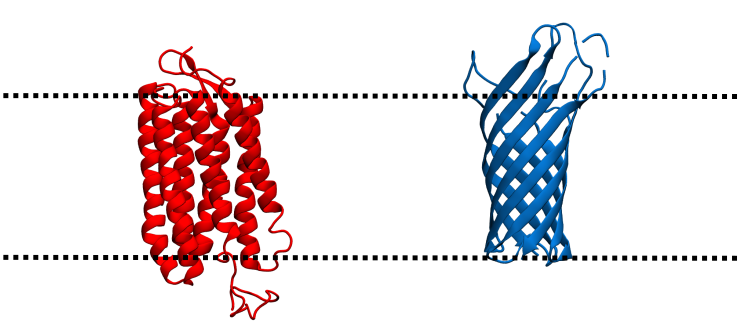
\includegraphics[width=\textwidth]{figures/introduction/Fig1/fig1.pdf}
\end{center}
	\caption{$\alpha$-helical versus $\beta$-barrel membrane protein}
Two representative structures of $\alpha$-helical and $\beta$-barrel membrane proteins are shown. Structure of bacteriorhodopsin (PDB ID: 1X0S) monomer is on the left in red, and OmpA (PDB ID: 1BXW) is shown on the right in blue. Hypothetical membrane boundaries are drawn in dashed black lines
	\label{fig:intro_f1}
\end{figure}

Individual $\alpha$-helices can be stable in the membrane as long as sidechains are hydrophobic enough; however, $\beta$-strands are not stable in the membrane because of exposed unsatisfied hydrogen donors and acceptors from the peptide backbone. Due to this difference in secondary structure, $\beta$-barrel membrane proteins insert and fold concurrently whereas $\alpha$-helical membrane proteins will insert one helix at a time and the helices rearrange to fold within the bilayer. In addition, $\beta$-barrel membrane proteins have been shown to fold reversibly from solution containing traditional denaturants such as urea and guanadine hydrochloride (GdnHCl) into lipids. (Fleming, Radford, Tamm, Rockwell) Because $\beta$-barrel membrane proteins can be monomeric and soluble in traditional denaturants, several proteins' (e.g. OmpA, OmpLA, OmpW, PagP) folding thermodynamics have been measured. In which, they found that they fold cooperatively by forming $\beta$ sheets at the lipid-water interface and insert. On the other hand, $\alpha$-helical membrane proteins are highly resistant to urea and GdnHCl, largely due to its hydrophobicity, and the denaturant of choice is sodium dodecyl sulfate (SDS) for folding studies of $\alpha$-helical membrane protein. With SDS, unfolded state of $\alpha$-helical membrane proteins still retain majority of its helicity. Because of this chemical property, most $\alpha$-helical membrane protein folding studies have focused on measuring folding thermodynamics and kinetics from SDS-unfolded states. 

The difference in folding mechanism is also reflected in how chaperones help these two classes of proteins fold. For $\beta$-barrel membrane proteins, BAM complexes have been shown to help them insert and fold by thinning the lipid bilayer thickness hence lowering the energy barrier to insert and fold. On the other hand, for $\alpha$-helical membrane proteins, ribosomes dock onto the SEC translocons and single helices are synthesized and inserted into the membrane one at a time as shown in \textbf{Figure \ref{fig:intro_f2}}. Many advances have been made in the field of $\beta$-barrel membrane proteins and there are excellent reviews available. (Fleming, Rockwell, Radford) Here in this thesis, the focus will be on the folding of $\alpha$-helical membrane proteins.

\begin{figure}[!ht]
\begin{center}
	\includegraphics[width=\textwidth]{figures/introduction/Fig2/two_stage.pdf}
\end{center}
	\caption{Two-stage folding process for membrane protein folding.}
The first stage of the membrane protein folding process is insertion, where single helices are synthesized and inserted into the bilayer one at a time. As noted above, the insertion process is different for \textit{in vivo} and \textit{in vitro}. However, upon insertion of helices into the membrane, folding within the membrane is thought to process via the same pathway. 
	\label{fig:intro_f2}
\end{figure}

$\alpha$-helical membrane protein folding process is generally divided into 2 distinct stages (\textbf{Fig. \ref{fig:intro_f2}}). The first stage of membrane protein folding is called insertion, where the protein gets inserted into the membrane with native-like secondary structures. The exact mechanism on how a single helix transfers from inside the SEC translocon into the bilayer is not well understood yet, but the transfer is thought to happen via a lateral gate that opens in the translocon. Regardless, the insertion process is largely determined by the hydrophobicity of the peptide segment. Using amino acid hydrophobicity scales and sliding window averages, transmembrane segments can be well predicted. Yet, the prediction of final overall topology is still a difficult task. For some systems like LacY, the overall topologies can be flipped by changing the lipid compositions \textit{in vivo} and \textit{in vitro}.

After successful insertion of helices into the membrane, the helices begin to undergo a rearrangement process, which is described as folding within the membrane. This process is determined by many different forces including protein-protein and protein-lipid interactions. The major driving force for helix-helix interactions are not clear. Polar sidechain burial was thought of as a driving force for helix-helix associations; however, it was found



\section{Potassium Channels}
Potassium channels are found in all kingdoms of life. From bacteria to humans, potassium channels regulate the flow of K+ ions across cell membranes. In prokaryotes, these channels are responsible for cell growth and survival. In addition, biofilm, which is a community of bacterial cells, the microorganisms use potassium channels to communicate with each other. In higher order organisms like humans, potassium channels are used to drive muscle contraction and neuronal signaling.

The first structure of potassium channel was solved in 1998 by Roderick MacKinnon's lab, which he was awarded the Nobel Prize in Chemistry for in 2003. The structure showed that the pore is formed by juxtaposition of 4 subunits along the symmetry axis. The pore is lined with oxygen atoms from the backbone of the selectivity filter residues. Thes oxygen atoms provide binding sites for K+ ions as they pass through the pore. 


\section{Potassium Channel Folding}

%%\newpage
%%The aims of my studies are:
%%\begin{itemize}
%%\item Determine the structural state of potassium channel monomers in lipid bilayers
%%\item Determine the folding pathway of potassium channels
%%\end{itemize}

%% END INTRODUCTION %%




%%% BEGIN CHAPTER 2 MICROARRAY %%%

%% Paper title page %%
\chapter[PLZF expression maps the early stages of ILC1 lineage \\ development]{PLZF expression maps the early stages of ILC1 lineage development}

% authors
Michael G. Constantinides\U{a}, Herman Gudjonson\U{b}, Benjamin D. McDonald\U{a}, Isabel E. Ishizuka\U{a}, Philip A. Verhoef\U{a}, Aaron R. Dinner\U{a,b,c}, and Albert Bendelac\U{a,1}
\\ \\
\U{a}Committee on Immunology,\\
\U{b}Institute for Biophysical Dynamics, and \\
\U{c}Department of Chemistry, University of Chicago, Chicago, IL 60637 
\\
\U{1}To whom correspondence should be addressed. Email\: abendela@bsd.uchicago.edu
\\ \\
Author contributions: M.G.C. and A.B. designed research; M.G.C., H.G., B.D.M., I.E.I., and P.A.V. performed research; M.G.C., H.G., A.R.D., and A.B. analyzed data; M.G.C. and A.B. wrote the paper; and H.G. performed bioinformatics analysis.
\\ \\
Published in PNAS March 11, 2015; doi:10.1073/pnas.1423244112

\newpage
\section{SIGNIFICANCE}
Diverse populations of group 1 innate lymphocytes, which exert critical early cytolytic functions against virally infected cells, have recently been discovered, raising issues of lineage relationships. We used expression of the transcription factor promyelocytic leukaemia zinc finger (PLZF) to identify the developmental intermediates of innate lymphoid cells type 1 (ILC1s), a subset of innate lymphoid cells that are particularly abundant in the liver, and demonstrated that this lineage arises from a distinct precursor, but that its development partially overlaps with established classical NK stages. Using microarray analysis, we defined a set of PLZF-dependent genes that may contribute to lineage divergence between ILC1s and classical NK cells.

\section{ABSTRACT}

Among the variety of tissue-resident NK-like populations recently distinguished from recirculating classical NK (cNK) cells, liver innate lymphoid cells (ILC) type 1 (ILC1s) have been shown to represent a distinct lineage that originates from a novel promyelocytic leukaemia zinc finger (PLZF)-expressing ILC precursor (ILCP) strictly committed to the ILC1, ILC2, and ILC3 lineages. Here, using PLZF-reporter mice and cell transfer assays, we studied the developmental progression of ILC1s and demonstrated substantial overlap with stages previously ascribed to the cNK lineage, including pre–pro-NK, pre-NK precursor (pre-NKP), refined NKP (rNKP), and immature NK (iNK). Although they originated from different precursors, the ILC1 and cNK lineages followed a parallel progression at early stages and diverged later at the iNK stage, with a striking predominance of ILC1s over cNKs early in ontogeny. Although a limited set of ILC1 genes depended on PLZF for expression, characteristically including \textit{Il7r}, most of these genes were also differentially expressed between ILC1s and cNKs, indicating that PLZF together with other, yet to be defined, factors contribute to the divergence between these lineages.

\section{INTRODUCTION}

NK cells represent the longest and best studied population of innate lymphocytes, whose roles in host defense against infections, particularly viral infection by cytomegalovirus, and in tumor or transplant rejection have been extensively characterized \cite{sun2009,yokoyama2004,vivier2011}. The core NK program is based on a panoply of NK-lineage receptors specific for MHC and MHC-like ligands that are induced by stress and infection to trigger perforin- and granzyme-mediated cytolysis of target cells and secretion of type 1 cytokines. This program is controlled in part by the transcription factor T-bet, the related factor eomesodermin, and the cytokine IL-15.

NK cells were long considered to be a single lineage phenotypically characterized by the surface \CDte\UM NK1.1\UP DX5\UP{} profile of its mature product. However, several recent studies have revealed the existence of distinct subpopulations of NK-like cells that, unlike the recirculating classical NK (cNK) cells found in spleen, blood, and lymph nodes, exhibited the unusual property of long-term residence in particular tissues, including liver, intestinal epithelium, uterus, skin, and salivary glands \cite{sojka2014,yokoyama2013,peng2013,cortez2014, fuchs2013,sojka2014review}. For example, in parabiotic pairs of CD45\UM{} congenic mice, a fraction of \CDte\UM NK1.1\UP liver cells were found to be tissue-resident rather than recirculating cells (6). The resident cells were further distinguished from cNK cells by the expression of the TNF family member TNFSF10 (TRAIL), the presence of high levels of integrin $\alpha$1 chain (CD49a), the absence of integrin $\alpha$2 (CD49b, stained by the DX5 antibody), and the expression of CD160, a receptor for epithelium-expressed HVEM \cite{sojka2014,peng2013,fuchs2013,klose2014}. Whereas, like cNKs, the liver-resident cells expressed T-bet and were endowed with cytolytic and type 1 cytokine secretion properties, they characteristically lacked eomesodermin and expressed some level of surface IL7R$\alpha$ chain \cite{sojka2014,klose2014,daussy2014}. Although their DX5\UM phenotype initially suggested they were immature NK cells \cite{takeda2005,gordon2012,vosshenrich2013}, further studies based on fate mapping and cell transfers into \Ragrg hosts established that they represented a different lineage, originating from a small subset of lineage (Lin)\UM IL7R$\alpha$\UP \ab\U{high} Id2\U{high} bone marrow or fetal liver cells that transiently but characteristically expressed high amounts of the transcription factor promyelocytic leukaemia zinc finger (PLZF) \cite{klose2014,constantinides2014}. This PLZF-expressing precursor was termed the ILC precursor (ILCP) because it also generated ILC2s and ILC3s, but, importantly, generated only few cNK-like cells and did not give rise to LTis, B, or T cells \cite{constantinides2014}. Consistent with these findings, most innate lymphoid cells type 1 (ILC1s) were fate-mapped by PLZF, whereas, in contrast, cNKs were generally not fate-mapped, with the notable exception of a small fraction of cNKs, which perhaps originated from ILCPs that retained some cNK potential or, alternatively, were derived from rare cNK precursors that might express low level of PLZF. Thus, these findings altogether supported the notion that ILC1s and cNKs primarily originated from different precursors. Furthermore, although there remain a few discrepancies in the description of these cells by different groups, in particular regarding the degree of requirement for the transcription factor Nfil3 \cite{sojka2014,yu2014}, it seems clear that the liver-resident NK cells described by Yokoyama and coworkers are largely identical to liver ILC1s \cite{sojka2014}.

The early stages of NK cell development have long been elusive. A \CDte\UM CD122 (IL2R$\beta$)\UP NK1.1\UM{} NK precursor (NKP) subset was first identified based on its ability to generate NK1.1\UP cells upon single cell culture in vitro, albeit with a relatively low clonal frequency of $\sim$1 in 12 \cite{kim2002,rosmaraki2001}. More recent studies, however, have refined the phenotype of these precursors based on the coexpression of CD122 with CD127 (IL7R$\alpha$), CD244, and CD27, identifying a refined NKP (rNKP) as well as an earlier, so-called pre-NKP stage, with a similar phenotype, except for low or absent CD122 \cite{fathman2011}. At the single cell level, both of these populations could generate \CDte\UM NK1.1\UP{} clones at a high frequency of $\sim$1 in 2 in culture with OP9 stromal cells and a mixture of the cytokines SCF, Flt3L, IL-7, and IL-15. In addition, after in vivo transfer into \Ragrg hosts, both populations generated exclusively \CDte\UM NK1.1\UP{} cells in the spleen and liver. Another study used an Id2-GFP reporter strain to identify a population of Lin\UM Id2\U{high} Sca1\UP CD117 (cKit)\U{int/--} CD135 (Flt3)\UM IL7R$\alpha$\UP{} cells, termed pre–pro-NKs \cite{carotta2011}, that generated \CDte\UM NK1.1\UP cells at a frequency of $\sim$1 in 2 upon single-cell culture in vitro with OP9 cells and a mixture of IL-7 and IL-15.

In this study, we used PLZF-IRES-GFPCre reporter mice and cell transfers to examine whether some of these early stages of development might be intermixed with, or reassigned to, ILC1s. We demonstrated considerable heterogeneity, with precursors to ILC1s but also ILC2s and ILC3s present in various proportions at different stages. Furthermore, by transcriptional analysis of PLZF-deficient ILC1s compared with WT ILC1s and cNKs, we identified a PLZF-dependent contribution to the genetic program that differentiates ILC1s from cNKs, which included the characteristic expression of the IL7R$\alpha$ chain. The results help redefine and clarify the early stages of ILC and cNK development and the contribution of PLZF to the divergence of these lineages.

\section{RESULTS}

\subsection{Early NK1.1\UM{} Stages of Development}

We used PLZF-IRES-GFPCre mice to report and fate-map PLZF expression in lymphoid compartments. We previously established that GFP faithfully reported PLZF expression in the hematopoietic compartment, with high levels of expression in ILCP and in NKT cells, but not in other lymphoid subsets \cite{constantinides2014}. However, in fate-mapping experiments based on the ROSA26-fl-STOP-fl-YFP allele, we reported that, whereas a majority of mature ILCs and NKT cells were YFP\UP, as expected, $\sim$30\% of other hematopoietic cells were also YFP\UP, including T, B, myeloid cells, and early hematopoietic cell precursors such as early HSC, LMPP, and CLP cells. This indiscriminate background mapping occurred before hematopoiesis, likely in early embryonic stem cells, because it was readily abrogated in radiation chimeras reconstituted with sorted YFP-negative Lin\UM Sca1\UP cKit\UP (LSK) precursors extracted from PLZF-IRES-GFPCre\UP ROSA26-fl-STOP-fl-YFP mice \cite{constantinides2014}. In the experiments reported below, we used these chimeras, termed YFP-negative chimeras, to faithfully fate-map PLZF expression in the hematopoietic system.

To precisely track the expression of PLZF side by side with fate-mapping at different stages of lymphoid development, we compared GFP expression in straight PLZF-IRES-GFPCre\UP mice with YFP expression in YFP-negative chimeras (Fig. \ref{fig:chap2_F1}). We zoomed in on the pre-NKP and rNKP stages, identified by their Lin\UM IL7R$\alpha$\UP CD27\UP CD244\UP CD117 (cKit)\U{int/low} Flt3\UM{} profile, with the pre-NKP expressing weak or absent CD122 (IL2R$\beta$), and the rNKP expressing high CD122 \cite{fathman2011} as gated in Fig. \ref{fig:chap2_F1}A. Both pre-NKPs and rNKPs were previously shown to selectively reconstitute \CDte\UM NKp46\UP NK1.1\UP Ly49D\UP Ly49H\UP cNK cells in the spleen and liver of \Ragrg mice after in vivo transfer, but a detailed analysis of markers that can identify ILC1s, such as CD49a, DX5, TRAIL, CD127 (IL7R$\alpha$), or eomesodermin, was not reported \cite{fathman2011}. Whereas CLPs failed to express either GFP or YFP, as expected, we found that nearly half of pre-NKPs expressed high amounts of GFP (Fig. \ref{fig:chap2_F1}A), a property previously shown to be restricted to the ILCP \cite{constantinides2014}. Furthermore, at the subsequent rNKP stage, the expression of GFP was down-modulated, both in frequency and in intensity, whereas YFP fate-mapping increased from 15 to 36\% on average (Fig. \ref{fig:chap2_F1}A). These findings suggested that cells with the “pre-NKP” phenotype in fact included a large fraction of PLZF-expressing ILCPs, which subsequently down-regulated PLZF and began to exhibit fate-mapping as they progressed into what was previously described as the “rNKP” stage.

%% Chapter 2 Figure 1 NKP Populations %%
\begin{figure}[p]
\begin{center}
	\includegraphics[width=\textwidth]{figures/chapter2/F1}
\end{center}
	\caption{Pre-NKPs and rNKPs are heterogeneous populations.} 
	(A) Gating strategy for CLPs (CD122\UM Flt3\UP), pre-NKPs (CD122\UM Flt3\UM), and rNKPs (CD122\UP Flt3\UM) among Lin\UM Ly6D\UM CD27\UP CD244\UP IL-7R$\alpha$\UP{} bone marrow cells (left four dot plots). Histograms show expression of GFP (reporting PLZF; Top) by the indicated cell types from PLZF\U{GFPcre+/+} (filled gray) and wild-type (open) mice and YFP (reporting fate-mapping by PLZF; Bottom) by the same cell types in YFP-negative chimeras (radiation chimeras reconstituted with YFP\UM Lin\UM Sca-1\UP cKit\UP (LSK) bone marrow cells from PLZF\U{GFPcre+/--} ROSA26-YFP mice). Bar graphs show summary of results (mean $\pm$ SEM). (B) FACS analysis of Ly6D\UM bone marrow cells from adult WT (Top) and PLZF\U{GFPcre+/+} (Middle) mice. Bottom depicts the same results in histogram form with GFP\U{high} (open) and GFP\UM (filled gray) Ly6D\UM bone marrow cells from adult PLZF\U{GFPcre+/+} animals. (C) Expression of GFP and \ab{} by the indicated cell types from PLZF\U{GFPcre+/+} mice. Representative of 3–8 mice analyzed in three or more independent experiments. *$P < 0.05$.
	\label{fig:chap2_F1}
\end{figure}

We therefore extended the comparison between the GFP\U{high} fraction of pre-NKPs and the previously defined ILCPs. Gating on GFP\U{high} cells in the entire bone marrow compartment, we found that these cells not only uniformly expressed the Lin\UM \ab\U{high} CD127 (IL7R$\alpha$)\U{high} CD117 (c-Kit)\UP profile, as previously described for ILCPs, but also were negative for CD135 (Flt3) and positive for CD27 and CD244 (Fig. \ref{fig:chap2_F1}B), the key markers of pre-NKPs \cite{fathman2011}. In contrast, the GFP-negative fraction of pre-NKPs lacked \ab{} expression (Fig. \ref{fig:chap2_F1}C). Because the transition between pre-NKPs and rNKPs is marked by the up-regulation of CD122, we reexamined CD122 expression with a bright antibody-biotin and streptavidin-phycoerythrin combination to detect low quantities of this protein on the cell surface. Indeed, we found that ILCPs expressed variable amounts of surface CD122 that ranged from negative to intermediate and, thus, might include cells already committing to the ILC1 sublineage (Fig. \ref{fig:chap2_F1}B, \textit{Far Right}).

Thus, we conclude that the previously described pre-NKP population is composed of a mixture of ILCPs (precursors to ILC1s, ILC2s, and ILC3s) and cNK precursors. These two fractions can be distinguished by their differential pattern of expression of PLZF and \ab. The distinct progenies of these two fractions can be inferred from transfer experiments showing that the unfractionated pre-NKPs generated classical NK cells in the spleen \cite{fathman2011}, whereas the PLZF\UP \ab\UP (ILCP) fraction did not \cite{constantinides2014}. In retrospect, the failure to observe significant NK1.1\UM progeny (i.e., ILC2 and ILC3) after transfer of pre-NKPs into \Ragrg hosts in the study by Fathman et al. \cite{fathman2011}, is consistent with their focus on spleen and liver, whereas ILC2s and ILC3s predominate in the intestinal lamina propria.

We also examined the Lin\UM Sca1\UP CD117 (cKit)\U{int/--} CD135 (Flt3)\UM IL7R$\alpha$\UP cell, which was proposed to be an early NK precursor, termed pre–pro-NK \cite{carotta2011}. Strikingly, we found uniform but low expression of GFP contrasting with a high frequency of YFP fate-mapping, suggesting that a large fraction of these cells had, in fact, originated from ILCPs and down-regulated PLZF (Fig. \ref{fig:chap2_S1}). Because the majority of these cells also expressed CD25, ICOS, and T1/ST2, the combination of which is highly characteristic of ILC2s, we concluded that they mostly represented late developmental intermediates of ILC2s termed immature ILC2s (iILC2 or LSIG), rather than cNK precursors, consistent with their reported Id2high profile \cite{hoyler2012}. Indeed, cell transfers into \Ragrg hosts have demonstrated that this precursor population exclusively generates mature ILC2 in vivo \cite{hoyler2012}.

\subsection{Immature NKs}

We next examined the so-called immature NK (iNK) cells, which are defined by expression of NKp46 and NK1.1, but not DX5. Although these cells were previously considered to be developmental intermediates of the cNK lineage before acquisition of DX5 \cite{yokoyama2004}, recent reports have emphasized that a fraction of iNKs expressed a phenotype similar to that of mature ILC1s, including expression of IL7R$\alpha$ and CD49a, but neither CD49b (DX5) nor eomesodermin \cite{sojka2014,klose2014,diefenbach2014}. In one study, transfer of eomesodermin-negative iNKs into \Ragrg hosts reconstituted liver ILC1s but not cNKs \cite{klose2014}. We found that nearly 80\% of iNKs, defined by their \CDte\UM CD122\UP NKp46\UP NK1.1\UP DX5\UM{} profile, were YFP\UP, but these cells did not express GFP, suggesting that a large proportion had originated from ILC1 rather than from cNK precursors (Fig. \ref{fig:chap2_F2}A). We further showed that the PLZF fate-mapped iNKs (isolated from YFP-negative chimeras) gave rise exclusively to CD49a\UP DX5\UM (ILC1s) but not to CD49a\UM DX5\UP (cNKs) liver cells after transfer into \Ragrg recipients (Fig. \ref{fig:chap2_F2}B). In contrast, CD45-congenic CLPs (coinjected with the YFP\UP iNKs) generated both cNKs and ILC1s in the liver (Fig. \ref{fig:chap2_F2}B). We also purified bone marrow \CDte\UM NKp46\UP NK1.1\UP DX5\UM{} iNKs, irrespective of their PLZF fate-mapping, and transferred them into \Ragrg hosts, to test whether they contained cNK precursors. Although these cells generated a majority of ILC1s, consistent with the predominance of ILC1 precursors, we also observed a substantial fraction of cNKs (Fig. \ref{fig:chap2_F2}B). Thus, \CDte\UM NKp46\UP NK1.1\UP DX5\UM{} bone marrow cells, previously termed iNKs, are a mixture of both ILC1 and cNK lineage cells, with a strong predominance of ILC1s. Upon stimulation with ionomycin and PMA, the bone marrow \CDte\UM NKp46\UP NK1.1\UP DX5\UM cells produced significantly less IFN-$\gamma$ than their liver counterpart, further supporting the notion that they represented immature ILC1s (iILC1s) (Fig. \ref{fig:chap2_F2}C).

%% Chapter 2 Figure 2 ILC1 and cNK precursors %%
\begin{figure}[p]
\begin{center}
	\includegraphics[width=0.4\textwidth]{figures/chapter2/F2}
\end{center}
	\caption{A majority of bone marrow NK1.1\UP DX5\UM “immature NKs” are ILC1 rather than cNK precursors.} 
	(A) Gating strategy for DX5\UM (NK1.1\UP DX5\UM) and DX5\UP (NK1.1\UP DX5\UP) populations among Lin\UM CD122\UP NKp46\UP{} bone marrow cells (left four dot plots). Histograms show expression of GFP (reporting PLZF; Top) by the DX5\UM{} and DX5\UP{} populations from PLZF\U{GFPcre+/+} (filled gray) and WT (open) mice and YFP expression (reporting PLZF fate-mapping; Bottom). Bar graphs show summary of results (mean $\pm$ SEM) for bone marrow DX5\UM{} and DX5\UP{} cells (as gated) and for liver DX5\UM (\CDte\UM TCR$\beta$\UM NK1.1\UP DX5\UM) and DX5\UP (\CDte\UM TCR$\beta$\UM NK1.1\UP DX5\UP) populations. Data representative of 3–5 mice analyzed in three independent experiments. (B) CD45.2 \Ragrg mice were injected with a mixture of 750 CD45.1 CLPs + 1,500 YFP\UP Lin\UM CD122\UP NKp46\UP NK1.1\UP DX5\UM bone marrow cells from YFP\UM chimeras or with 1,500 CD45.1 Lin\UM CD122\UP NKp46\UP NK1.1\UP DX5\UM bone marrow cells alone, as indicated. The progeny of these populations within the liver was analyzed 3–4 wk later by FACS. Bar graphs show summary of results (mean $\pm$ SEM). Representative of 3–5 chimeras analyzed in two independent experiments. (C) The Lin\UM CD122\UP NKp46\UP NK1.1\UP DX5\UM{} bone marrow (BM DX5\UM) and \CDte\UM TCR$\beta$\UM NK1.1\UP DX5\UM{} liver (liver DX5\UM) populations were sorted from WT mice and stimulated with PMA (20 ng/mL) and ionomycin (5 $\mu$g/mL) for 4 h in the presence of 1x GolgiStop, and IFN-$\gamma$ production was analyzed by intracellular FACS staining (filled gray). Control histograms (open) are from unstimulated cells. Results from three independent experiments summarized in the bar graph (mean $\pm$ SEM). *$P < 0.05$.
	\label{fig:chap2_F2}
\end{figure}

Altogether, our analysis of the developmental stages of ILC1s and cNKs suggests a new model whereby these lineages originate from distinct precursors, distinguished by the expression of PLZF and \ab, before undergoing a parallel sequence of progressive steps encompassing previously described populations and diverging between iNKs and iILC1s as proposed in Fig. \ref{fig:chap2_S2}.

\subsection{Predominance of ILC1s Early in Ontogeny}

Tissue-resident ILC1s are reminiscent of the early waves of tissue-resident \gdT cells that populate tissues such as skin, uterus, intestine, liver, and lung in the newborn (23). These tissue-resident \gdT cells express semiinvariant TCRs and are thought to represent a first line of defense in the perinatal period, before the generation of their blood recirculating counterparts, which have a more diverse repertoire. Indeed, we found that a great majority of \CDte\UM NK1.1\UP{} cells in both embryonic day (E)16 fetal liver and in 1-wk-old liver were YFP\UP fate-mapped, expressed CD49a and TRAIL, and lacked eomesodermin, whereas CD49a\UM TRAIL\UM eomesodermin\UP{} cNK cells appeared later in ontogeny between weeks 1 and 3, and were characterized by lower YFP fate-mapping (Fig. \ref{fig:chap2_F3}). Note that to study fetal and newborn hematopoiesis, these experiments used the straight PLZF-IRES-GFPCre crossed to ROSA-fl-STOP-fl-YFP mice, rather than the YFP-negative adult bone marrow chimeras. This experimental necessity explains in part the higher frequency of YFP labeling in cNKs, due to background labeling before the hematopoietic stem cell stage. Surprisingly, liver ILC1s tended to coexpress DX5 in fetal life, but not after birth, emphasizing that DX5 expression may not always be a reliable marker of cNKs. Altogether, these results therefore demonstrate that ILC1s strongly predominate over cNK cells in perinatal life, whereas cNK cells achieve greater frequency in adults.

%% Chapter 2 Figure 3 fetal ILC1 and cNK %%
\begin{figure}[p]
\begin{center}
	\includegraphics[height=0.5\textheight]{figures/chapter2/F3}
\end{center}
	\caption{Predominance of ILC1s over cNKs in the fetal and newborn liver.} 
	 FACS analysis of hepatic lymphocytes isolated from WT or PLZF\U{GFPcre+/--} ROSA26-YFP mice at E16 or at 1 and 3 wk after birth, as indicated. At Bottom, dot plots are divided into CD49a\UP{} and CD49a\UM{} fractions and the numbers indicate the percentages of YFP\UP{} and YFP\UM{} cells within each of these gates. All dot plots, except on the third row, are obtained from the same samples. Representative of 4–5 mice for each time point, analyzed in two independent experiments.
	\label{fig:chap2_F3}
\end{figure}

Impact of PLZF on ILC1 Development and Maturation. We previously showed that PLZF-deficient ILC1s were decreased fourfold compared with their wild-type counterparts in the liver of competitive bone marrow chimeras \cite{constantinides2014}. By microarray analysis, we found that ILC1s isolated from the liver of PLZF-deficient mice exhibited a limited set of changes compared with those of wild-type littermates, because only 229 genes had altered expression by more than 1.4-fold (Fig. \ref{fig:chap2_F4}A). In contrast, and similar to a recent study \cite{peng2013}, $>$2,000 genes exhibited differential expression between liver cNK cells and ILC1s, indicating that, as expected, the differences between cNKs and ILC1s do not solely depend on PLZF. Strikingly, however, 59\% of the PLZF-dependent genes in ILC1s were also differentially expressed between ILC1s and cNKs, a highly significant overlap ($P = 2.7 \times 10^{−93}$ by hypergeometric test). Because ILC1s and cNKs differ by their history of PLZF expression, these differentially expressed genes may be involved in the divergence between these two lineages. For example, PLZF-deficient ILC1s showed decreased expression of CD127 (IL7R$\alpha$), both at the mRNA level by microarray analysis and at the protein level by flow cytometry (Fig. \ref{fig:chap2_F4} B and C). IL7R$\alpha$ is expressed in the hematopoietic precursors to both ILC1s and cNKs, but its expression is characteristically maintained only in mature ILC1s \cite{diefenbach2014}. Although the role of IL7R$\alpha$ in ILC1 biology is not fully understood, because mature ILC1s seem mostly dependent on IL15 for their maintenance \cite{sojka2014}, it may be important for optimal survival during a developmental window, before expression of the IL15 receptor. Thus, the conspicuous defect in IL7R$\alpha$ expression in PLZF-deficient ILC1s might contribute in part to their decreased frequency. Other ILC1 genes that depended on PLZF and were not expressed by cNKs included \textit{Mmp9}, \textit{Klrb1b}, \textit{Klrk1}, and \textit{Tnfrsf25}, as well as \textit{Cd3g} and \textit{Cd3e}, which were previously reported to be expressed by fetal but not adult NK cells \cite{lanier1992}. This expression of Cd3 genes may reflect the predominance of ILC1s over cNKs in the fetus. Most of the genes that were differentially expressed between wild-type ILC1s and PLZF-deficient ILC1s as well as between wild-type ILC1s and cNKs cells showed concordant changes in the two comparisons (Fig. \ref{fig:chap2_F4}B, upper right and lower left quadrants), although there were examples of opposite variations (Fig. \ref{fig:chap2_F4}B, upper left and lower right quadrants), for example for \textit{Il18r1}. Importantly, several of the key genes that were differentially expressed between cNKs and ILC1s, including \textit{Eomes}, Itga1 encoding \textit{CD49a}, \textit{Tnfsf10} encoding TRAIL, \textit{Sell} encoding CD62L, \textit{Edg8} encoding S1P5, and \textit{Cxcr6}, did not seem to be influenced by PLZF.

%% Chapter 2 Figure 4 microarray ILC1 and cNK %%
\begin{figure}[p]
\begin{center}
	\includegraphics[width=\textwidth]{figures/chapter2/F4}
\end{center}
	\caption{Most PLZF-dependent genes in ILC1s are also differentially expressed between ILC1s and cNKs.} 
	 Shown is a comparison of changes in gene expression due to PLZF deficiency in ILC1s (ILC1 WT/PLZF KO) and changes in gene expression between ILC1s versus cNKs (ILC1/cNK). (A) Venn diagram. The P value for 134/229 PLZF-dependent genes to be part of the 2,179 genes differentially expressed between ILC1s and cNKs is $2.7 \times 10^{−93}$ by hypergeometric test. (B) Scatter plot. Dotted lines delineate the 1.4-fold change threshold. Select immune genes are highlighted. (C) FACS analysis of IL7R$\alpha$ expression by liver ILC1s (DX5\UM) and cNKs (DX5\UP) from PLZF\U{--/--} (open) and WT littermates (filled gray), with T cells as positive controls (\CDte\UP NK1.1\UM). Mean fluorescence intensity (MFI) is indicated in black for PLZF\U{--/--} and gray for WT. Representative of 4 WT and 4 PLZF\U{--/--} littermates examined in two separate experiments.
	\label{fig:chap2_F4}
\end{figure}

\section{DISCUSSION}

This study uses PLZF reporting and fate-mapping to identify developmental intermediates in the ILC1 lineage pathway and to define their relationship with previously proposed stages of cNK development. Whereas the history of expression of PLZF and \ab{} clearly distinguished ILC1 from cNK precursors, the subsequent developmental intermediates appeared to be intermixed within the rNKP and iNK stages, which were previously assigned solely to cNKs. The earlier, pre-NKP stage appeared to be an even more complex mixture of PLZF-expressing ILCPs, which can give rise to ILC1s, ILC2s, and ILC3s, and of PLZF-negative cNK precursors. In contrast, the so-called “pre–pro-NK” cells, previously shown to generate NK1.1\UP{} cells in single-cell culture with OP9 and IL-15, include a majority of immature ILC2s, suggesting that these cells might exhibit a degree of plasticity in forced cytokine environments, as reported recently for more mature ILC lineages \cite{klose2013,huang2015}.

The earliest committed precursor to the cNK lineage has not been physically identified yet. Although the PLZF\UM \ab\UM{} fraction of pre-NKPs is likely associated with the cNK lineage, recent studies using transfer experiments into \Ragrg hosts suggested that an earlier cNK precursor might be found at a post-CLP stage defined by a Lin\UM IL7R$\alpha$\UP \ab\U{high} Id2\U{low} PLZF\U{low/neg} profile \cite{klose2014,yu2014}. These cells might then rapidly down-regulate \ab{} to become pre-NKPs in the cNK pathway. Thus, whereas ILC1s and cNKs both require NFIL3 and Tox at an early phase of their development, the divergence between these lineages is associated with the differential regulation of \ab{} and PLZF, and possibly other factors such as Id2 and Gata3, which are also expressed at very high levels in ILCPs \cite{constantinides2014}. The divergence between these lineages and the parallel stages of their development are depicted in Fig. \ref{fig:chap2_S2}.

Our study demonstrates that PLZF accompanies but is not absolutely required for this divergence. Indeed, PLZF has a detectable impact, as demonstrated by the observation that most of the PLZF-dependent genes in ILC1s, including the characteristic Il7r, are also differentially expressed between ILC1s and cNKs. However, this impact is relatively modest compared, for example, with NKT thymocyte development, where PLZF is absolutely essential for the acquisition of the T-helper polarized effector programs, which closely mirrors the trifurcation of ILCPs into ILC1, ILC2, and ILC3 lineages. This surprising difference may reflect the presence of redundant gene(s) in ILCPs or, alternatively, may suggest that PLZF-deficient ILC1s are expanded from a fraction of precursors that overcome defective survival signals, for example through the IL7 receptor, but are otherwise relatively normal. Future studies of the redefined early stages of cNK and ILC development should help unravel the transcriptional events controlling these innate lymphoid lineages and elucidate the molecular basis of their divergence.

\section{METHODS}

\textit{Mice}. C57BL/6J (stock no. 000664), B6.SJL-\textit{Ptprc}\U{a} \textit{Pepc}\U{b}/BoyJ (CD45.1; stock no. 002014), and B6.129 × 1-Gt(ROSA)26Sor\U{tm1(EYFP)Cos}/J (stock no. 006148) mice were obtained from The Jackson Laboratory, whereas B6.Rag2\U{tm1Fwa} II2rg\U{tm1Wjl} (\Ragrg, stock no. 4111) mice were obtained from Taconic. The PLZF\U{GFPcre} strain has been described (15). PLZF\U{--/--} mice were a gift from P. P. Pandolfi, Beth Israel Deaconess Medical Center, Boston, and were backcrossed to C57BL/6J for at least nine generations. Unless noted otherwise, animals were 4–10 wk of age when analyzed and were compared with littermate controls obtained from crosses between heterozygous breeders. For fetal experiments, the morning a vaginal plug was observed was considered E0. Mice were housed in a specific pathogen-free environment at the University of Chicago, and experiments were performed in accordance with the guidelines of the Institutional Animal Care and Use Committee.
\\
\textit{Preparation of Cell Suspensions}. Spleen and liver were mechanically dissociated through 70-$\mu$m filters, and bone marrow was isolated by gently crushing femurs and tibias before filtration. Following dissociation, each liver was centrifuged at 400 × g for 5 min, resuspended in 5 mL of 40\% (vol/vol) Percoll (Sigma-Aldrich), and then centrifuged at 800 × g for 10 min. The supernatant was aspirated and the cell pellet was resuspended in HBSS (Gibco) containing 0.25\% BSA (Sigma-Aldrich) and 0.65 mg/L sodium azide (Sigma-Aldrich).
Flow Cytometry. Cell suspensions were incubated with purified anti-CD16/32 (clone 93) for 10 min on ice to block Fc receptors. Fluorochrome- or biotin-labeled monoclonal antibodies (clones denoted in parentheses) against \ab{} (DATK32), B220 (RA3-6B2), \CDte{} (145-2C11), CD4 (RM4-5 or GK1.5), CD8$\alpha$ (53-6.7), CD11b (M1/70), CD11c (N418), CD19 (6D5), CD25 (PC61), CD27 (LG.7F9), CD45.1 (A20), CD45.2 (104), CD49a (HM$\alpha$1), CD122 (5H4 or TM-$\beta$1), CD160 (7H1), CD244 (2B4), cKit (2B8), DX5 (DX5), Eomes (Dan11mag) Flt3 (A2F10), Gr-1 (RB6-8C5), ICOS (C398.4A), \IFNg (XMG1.2), IL-7R$\alpha$ (A7R34), Ly-6D (49-H4), NK1.1 (PK136), NKp46 (29A1.4), Sca-1 (D7), T1/ST2 (D1H9), TCR$\beta$ (H57-597), Ter-119 (TER-119), Thy1.2 (53-2.1) and TRAIL (N2B2) were purchased from BD Biosciences, BioLegend, eBioscience, or R\& D Systems. To exclude dead cells, 4',6-diamidino-2-phenylindole (DAPI; Molecular Probes) was added to all live samples. For intracellular staining, cells were fixed with 4\% paraformaldehyde and permeabilized by using the Foxp3 Transcription Factor Staining Buffer Set (eBioscience). Cells were run on an LSRII (BD Biosciences) or sorted by using a FACS Aria II (BD Biosciences) and analyzed by using FlowJo software (Tree Star). Collected events were gated on DAPI− lymphocytes and doublets were excluded.
Unless specified otherwise, CLPs were gated Lin\UM Ly6D\UM CD244\UP CD27\UP IL-7R$\alpha$\UP Flt3\UP CD122\UM{} (19), pre-NKP were gated Lin\UM Ly6D\UM CD244\UP CD27\UP IL-7R$\alpha$\UP Flt3\UM CD122\U{low/neg} (19), rNKP were gated Lin\UM Ly6D\UM CD244\UP CD27\UP IL-7R$\alpha$\UP Flt3\UM CD122\U{high} (19), pre–pro-NK were gated Lin\UM Sca-1\UP cKit\U{low} IL-7R$\alpha$\UP Flt3\UM{} (20), bone marrow DX5\UM{} cells were gated Lin\UM CD122\UP NK1.1\UP NKp46\UP DX5\UM{} (14), bone marrow DX5\UP cells were gated Lin\UM CD122\UP NK1.1\UP NKp46\UP DX5\UP, liver DX5\UP cells were gated \CDte\UM TCR$\beta$\UM NK1.1\UP DX5\UP CD49a\UM, and liver DX5\UM{} cells were gated \CDte\UM TCR$\beta$\UM NK1.1\UP DX5\UM CD49a\UP. Lineage mixtures for pre-NKPs, rNKPs, and CLPs included antibodies against \CDte, CD11b, CD19, and NK1.1; for pre–pro-NK: \CDte, CD8$\alpha$, CD11b, CD19, Gr-1, and Ter119; for bone marrow NK1.1\UP subsets: \CDte, CD4, CD8$\alpha$, CD19, and Ter119.
\\
\textit{Bone Marrow Chimeras}. To generate YFP\UM chimeras, $5–10 \times 10^3$ LSK cells were sorted from the bone marrow of PLZF\U{GFPcre+/--} ROSA-YFP mice and injected retroorbitally into lethally irradiated (1,000 rads) CD45.1 recipients. Chimeras were analyzed 5–7 wk after reconstitution, gating on CD45.2\UP cells to exclude residual host cells.
\\
\textit{Isolation and Adoptive Transfer of Bone Marrow CLPs and NK1.1\UP{} Subsets}. For the isolation of CLPs from CD45.1 bone marrow, lineage\UP cells were first depleted by using an autoMACS (Miltenyi Biotec) after staining with biotin-conjugated antibodies against B220, \CDte, CD4, CD8$\alpha$, CD11b, CD11c, CD19, Gr-1, NK1.1, TCR$\beta$, and Ter119, followed by incubation with SAv microbeads (Miltenyi Biotec). CLPs were then sorted as DAPI\UM Lin\UM IL-7R$\alpha$\UP cKit\U{int} Sca-1\U{int} Flt3\U{high} to greater than 95\% purity by using a FACS Aria II (BD Biosciences). For the isolation of YFP\UP NK1.1\UP DX5\UM{} cells, bone marrow from YFP\UM{} chimeras (described above) was stained with APC-conjugated anti-NK1.1 antibody, bound to anti-APC microbeads (Miltenyi Biotec), subjected to double-column enrichment, and sorted as DAPI\UM Lin\UM CD122\UP NK1.1\UP NKp46\UP DX5\UM YFP\UP to greater than 95\% purity. For the isolation of NK1.1\UP DX5\UM{} cells, CD45.1 bone marrow was stained with APC-conjugated anti-NK1.1 antibody, bound to anti-APC microbeads, subjected to double-column enrichment, and sorted as DAPI\UM Lin\UM CD122\UP NK1.1\UP NKp46\UP DX5\UM to greater than 95\% purity. For the NK1.1\UP subsets, the lineage mixture antibodies used were as follows: \CDte, CD4, CD8$\alpha$, CD19, and Ter119.
Following isolation, 1,500 YFP\UP NK1.1\UP DX5\UM{} cells mixed with 750 CD45.1-congenic CLPs, or 1,500 CD45.1 NK1.1\UP DX5\UM{} cells alone were injected retroorbitally into sublethally irradiated (400 rads) 6- to 10-wk-old CD45.2 \Ragrg mice. Recipient mice were analyzed 3–4 wk after transfer.
\\
\textit{Isolation and in Vitro Stimulation of NK1.1\UP DX5\UM{} Cells}. Following enrichment using FITC-NK1.1 and anti-FITC microbeads (Miltenyi Biotec), NK1.1\UP DX5\UM cells were sorted as DAPI\UM Lin\UM NK1.1\UP NKp46\UP DX5\UM from the bone marrow or DAPI\UM \CDte\UM TCR$\beta$\UM NK1.1\UP NKp46\UP DX5\UM from the liver of WT mice ($>$95\% purity). For the bone marrow cells, the lineage mixture antibodies used were the following: \CDte, CD4, CD8$\alpha$, CD19, TCR$\beta$, and Ter119. Up to 10,000 sorted cells were resuspended in 500 $mu$L of RPMI medium 1640 (Cellgro) containing 10\% FCS (Biowest) and 1× GolgiStop (BD). Samples were stimulated with phorbol 12-myristate 13-acetate (PMA; 20 ng/mL) and ionomycin (5 $\mu$g/mL) for 4 h at 37 °C. Following the stimulation, samples were fixed and permeabilized by using the Cytofix/Cytoperm kit (BD).
\\
\textit{Microarray Analysis}. Liver lymphocytes from pools of PLZF\U{+/+} or PLZF\U{--/--} mice were sorted into ILC1s (\CDte\UM NK1.1\UP CD49a\UP DX5\UM) and cNKs (\CDte\UM NK1.1\UP CD49a\UM DX5\UP) and stored in TRIzol (Life Technologies). RNA was isolated by using the RNeasy mini kit (Qiagen), processed, and annealed to the mouse WG-6 array (Illumina). Illumina MouseWG-6 v2.0 Expression BeadChip data were quality-checked by using the lumi package \cite{du2008} and quality control metrics in the R/Bioconductor statistical software package (v3.0.0). Data were background corrected and normalized by variance-stabilizing transformation \cite{lin2008} followed by quantile normalization. Data were log2 transformed and fit to linear models by using the limma package \cite{smyth2005} for fold change comparison between groups. A fold-change cutoff of 1.4 was used to distinguish differentially expressed genes. Microarray data has been deposited with the National Center for Biotechnology Information Gene Expression Omnibus repository under the accession number GSE65898.
\\
\textit{Statistical Analysis}. Two-tailed Student’s t test was performed by using Prism (GraphPad Software) to determine whether data differed from the expected value. *$P < 0.05$.

\subsubsection{Acknowledgments}
This work was supported by NIH Grants R01 AI108643, AI038339, and HL118092 (to A.B.) and University of Chicago Digestive Diseases Research Core Center Grant P30 DK42086.

%% FIGURE NUMBERING %%
\renewcommand\thefigure{\thechapter.S\arabic{figure}} 

\newpage
\section{SUPPORTING INFORMATION}
\setcounter{figure}{0}

%% Chapter 2 Figure S1 pre-proNK and ILC2s %%
\begin{figure}[h]
\begin{center}
	\includegraphics[width=0.4\textwidth]{figures/chapter2/S1}
\end{center}
	\caption{Pre-pro-NKs contain a majority of immature ILC2s.} 
	 (A, Top) Expression of GFP (reporting PLZF) by the pre-pro-NK population (Lin\UM Sca-1\UP cKit\U{--/low} Flt3\UM IL-7R$\alpha$\UP) from PLZF\U{GFPcre+/+} (filled gray) and WT (open) mice. (Bottom) YFP expression (reporting fate-mapping by PLZF) in YFP-negative radiation chimeras. (B) Summary of results (mean $\pm$ SEM) shown in A. (C) FACS analysis of pre-pro-NK cells, stained for indicated markers (filled gray) or with isotype controls (open). Data representative of at least three mice analyzed in two or more independent experiments.
	\label{fig:chap2_S1}
\end{figure}

%% Chapter 2 Figure S2 Divergence diagram %%
\begin{figure}[p]
\begin{center}
	\includegraphics[width=\textwidth]{figures/chapter2/S2}
\end{center}
	\caption{Divergence and parallels in the development of ILC1s and cNKs.} 
	 The diagram highlights, within the shaded rectangle, the parallel progression sequence of ILC1 and cNK progenitors, with ILCP, ILC1P, and iILC1 previously included in, and now distinguished from, pre-NKP, rNKP, and iNK, respectively. The abbreviated names of developmental intermediates include CLP (common lymphoid precursor), \aLP (\ab\UP lymphoid precursor), CHILP (common helper innate lymphocyte precursor), ILCP (innate lymphoid cell precursor), ILC1P (ILC1 precursor), iILC1 (immature ILC1), pre-NKP (pre-NK precursor), rNKP (refined NKP), iNK (immature NK), and mNK (mature NK).
	\label{fig:chap2_S2}
\end{figure}

%% REVERT FIGURE NUMBERING %%
\renewcommand\thefigure{\thechapter.\arabic{figure}} 

%%% END CHAPTER 2 MICROARRAY %%%




%%% BEGIN CHAPTER 3 SINGLECELL %%%

%% Paper title page %%
\chapter[Single--cell analysis defines the divergence between the \\ innate lymphoid cell lineage and lymphoid tissue--inducer cell lineage]{Single--cell analysis defines the divergence between the innate lymphoid cell lineage and lymphoid tissue--inducer cell lineage}

% authors
Isabel E Ishizuka\U{1,2,6}, Sylvestre Chea\U{3,6}, Herman Gudjonson\U{1,4-6}, Michael G Constantinides\U{1,2}, Aaron R Dinner\U{4,5}, Albert Bendelac\U{1,2,7} and Rachel Golub\U{3,7}
\\ \\
\U{1}Committee on Immunology, University of Chicago, Chicago, Illinois, USA. 
\U{2}Department of Pathology, University of Chicago, Chicago, Illinois, USA. 
\U{3}Institut Pasteur, Immunology Department, Lymphopoiesis Unit, Inserm U668, University Paris Diderot, Paris, France. 
\U{4}Institute of Biophysical Dynamics, University of Chicago, Chicago, Illinois, USA. 
\U{5}Department of Chemistry, University of Chicago, Chicago, Illinois, USA. 
\U{6}These authors contributed equally to this work. 
\U{7}These authors jointly directed this work. 
\\
Correspondence should be addressed to A.B. (abendela@bsd.uchicago.edu).
\\ \\
Author contributions: I.E.I., H.G., M.G.C. and A.B. designed the experiments; I.E.I. performed single-cell sorting and culture experiments; S.C. designed and performed the lymphoid Biomark assay; H.G. performed computational analysis of the Biomark experiments; M.G.C. designed and performed experiments; A.R.D. supervised computational analysis; A.B. supervised experiments; R.G. supervised Biomark experiments; and I.E.I., H.G. and A.B. wrote the manuscript with contributions from all authors.
\\ \\
Published in Nature Immunology January 18, 2016; doi:10.1038/ni.3344

\newpage
\section{ABSTRACT}

The precise lineage relationship between innate lymphoid cells (ILCs) and lymphoid tissue–inducer (LTi) cells is poorly understood. Using single-cell multiplex transcriptional analysis of 100 lymphoid genes and single-cell cultures of fetal liver precursor cells, we identified the common proximal precursor to these lineages and found that its bifurcation was marked by differential induction of the transcription factors PLZF and TCF1. Acquisition of individual effector programs specific to the ILC subsets ILC1, ILC2 and ILC3 was initiated later, at the common ILC precursor stage, by transient expression of mixed ILC1, ILC2 and ILC3 transcriptional patterns, whereas, in contrast, the development of LTi cells did not go through multilineage priming. Our findings provide insight into the divergent mechanisms of the differentiation of the ILC lineage and LTi cell lineage and establish a high-resolution 'blueprint' of their development.

\section{INTRODUCTION}

Innate lymphocytes lack B cell or T cell antigen receptors and exert effector functions at mucosal barriers \cite{diefenbach2014,serafini2015}. These populations segregate into three general groups on the basis of their expression of the transcription factors T-bet, GATA-3 and \RORgt. However, there is considerable heterogeneity among T-bet-expressing group 1 lymphocytes, which comprise conventional (or classical) natural killer (NK) cells (cNK cells), group 1 innate lymphoid cells (ILC1 cells) and tissue-resident NK cells, and among \RORgt-expressing group 3 lymphocytes, which comprise CCR6\UP lymphoid tissue-inducer (LTi) cells and CCR6\UM ILC3 cells. In addition, some plasticity has been reported among CCR6\UM ILC3 cells, which can upregulate T-bet expression and acquire group 1 properties \cite{klose2013}, and among some populations of ILC2 cells, which can acquire group 3 properties \cite{huang2015}.

Lineage-tracing and cell-transfer studies have suggested that ILC1, ILC2 and ILC3 cells, but not LTi cells or cNK cells, are derived from a common dedicated precursor, the ILC precursor (ILCP), characterized by expression of the transcription factor PLZF \cite{constantinides2014}. Similar to the LTi precursor (LTiP), the ILCP originates from a lymphoid precursor that expresses the integrin \ab{} and is itself derived from the common lymphoid precursor (CLP). The Id2\U{hi} fraction of \ab\UP lymphoid precursors, called 'common helper innate lymphoid precursors' (CHILPs), is a heterogeneous population that includes the PLZF-expressing ILCPs as well as precursors of LTi cells \cite{klose2014}, but whether the CHILP population includes a common precursor of both ILCs and LTi cells or separate precursors of each lineage has not yet been determined. A study has suggested that cNK cells might originate from an earlier Id2\U{lo}CXCR6\UP fraction of \ab-expressing lymphoid precursors (\aLPs) \cite{yu2014}. Thus, the developmental relationships between these lineages remain incompletely established.

Several transcription factors, including Nfil3, Tox, Id2, GATA-3, TCF-1 (encoded by \textit{Tcf7}) and PLZF (encoded by \textit{Zbtb16}) \cite{constantinides2014,yu2014,xu2015,seillet2014,seehus2015, hoyler2012,serafini2014,yagi2014,yang2013,mielke2013,moro2010}, are required for the development of all or several of these innate lineages, which suggests they have an effect at a common precursor stage. However, partial defects, rather than complete defects, have often been reported in mice lacking these transcription factors, which suggests substantial redundancy and complexity of this early transcriptional network. Other transcription factors have been found to selectively affect individual ILC lineages, such as the effect of \RORa{} (encoded by \textit{Rora}), Bcl-11b and Gfi1 in ILC2 cells \cite{wong2012,spooner2013,walker2015}, which suggests more distal effects in the ILC-differentiation pathway. Precise understanding of the general hierarchy of expression of these factors is missing, however, which limits the design and interpretation of mechanistic studies aiming at delineating their interplay.

Here we used cultures of single cells purified from the fetal livers of a mouse reporter strain expressing green fluorescent protein (GFP) and Cre recombinase from the gene encoding PLZF (\textit{Zbtb16}-GFP-Cre) to precisely define the differentiation stages between CLP and ILC and to identify the stage of divergence between ILCs and LTi cells. We also performed multiplex quantitative single-cell transcriptional analysis of 100 lymphoid genes to characterize the complexity of molecular events associated with this differentiation pathway. We derived a high-resolution map and inferred a precise ordering of the induction of transcription factor expression and identified previously unknown stages of development before and after PLZF expression and the stage of bifurcation between the ILC lineage and LTi cell lineage. Notably, transcriptional priming for the different cytokine effector programs occurred at the ILCP stage itself through multilineage priming. In contrast, the LTiP proceeded to directly acquire its type 3 program without undergoing mixed transcriptional priming. Together our findings further define the dichotomy between ILCs and LTi cells and provide new insight into the stages and mechanisms of their development and the interplay of transcription factors that direct their differentiation.

\section{RESULTS}

\subsection{Bifurcation of \aLPs into ILCPs and LTiPs}
Lin\UM IL-7R$\alpha$\UP fetal liver cells (where lineage (Lin) is defined by a 'cocktail' of antibodies to \CDte, TCR$\beta$, CD19, CD11c, GR-1, Ter119 and NK1.1) included CLPs, identified by a Flt3\UP \ab\UM{} profile, and a cell population expressing \ab, which included the precursors to innate lymphoid lineage, thought to arise from the CLP (Fig. \ref{fig:chap3_F1}a). This \ab-expressing population was originally called '\aLP', but the identification of ILCPs and LTiPs among \aLPs prompted us to limit the designation of '\aLP' to the \ab-expressing cells that were neither ILCP nor LTiP but include their precursors \cite{serafini2015,moro2015}. We further subcategorized this \aLP population as an Flt3\UP subset and Flt3\UM subset to identify early precursors and late precursors, respectively. We detected these populations by flow cytometry among fetal liver cells obtained from the \textit{Zbtb16}-GFP-Cre reporter strain at embryonic day 15 (E15) (Fig. \ref{fig:chap3_F1}a). Among the Lin\UM IL-7R$\alpha$\UP \ab\UP{} population, the ILCPs were identified by GFP expression, and the LTiPs were identified by their GFP\UM CXCR5\UP profile \cite{constantinides2014,cherrier2012}. The LTiPs were clearly distinguishable from the other subsets in this staining, although a small fraction of these cells seemed to have low expression of GFP (Fig. \ref{fig:chap3_F1}a). As expected, only the LTiPs coexpressed the chemokine CCR6 and the coreceptor CD4 (Fig. \ref{fig:chap3_F1}b).

%% Chapter 3 Figure 1 aLP subpopulations %%
\begin{figure}[h]
\begin{center}
	\includegraphics[width=\textwidth]{figures/chapter3/F1}
\end{center}
	\caption{Identification of distinct subpopulations of \ab-expressing lymphoid precursors in fetal liver.} 
	(a) Flow cytometry of fetal liver cells from E15 Z \textit{Zbtb16}-GFP-Cre reporter mice after depletion of Lin\UP cells (expressing \CDte, CD11c, CD19, NK1.1, TCR$\beta$, Ter119 and GR-1) by magnetic bead–based cell separation and staining for IL-7R$\alpha$ (left), Flt3 and \ab{} (middle) and CXCR5 (right), for the identification of distinct subpopulations representing CLPs, \aLPs, LTiPs and ILCPs (middle and right) after gating on Lin\UM IL-7R$\alpha$\UP{} cells (left). Numbers adjacent to outlined areas indicate percent cells in each subpopulation. (b) Flow cytometry of ILCPs, LTiPs and Flt3\UM{} \aLPs stained for CCR6 or CD4. (c) Quantification of \aLPs, LTiPs and ILCPs in fetal liver at E12, E13 and E15. Each symbol represents an individual fetus; small horizontal lines indicate the mean. Data are representative of twelve independent experiments (a) or three experiments (b) or are pooled from two independent experiments (c).
	\label{fig:chap3_F1}
\end{figure}

Both LTiPs and ILCPs could already be detected at a low frequency among Lin\UM IL-7R$\alpha$\UP \ab\UP{} fetal liver cells at E12, the earliest time point of our analysis, and their absolute numbers increased five- to tenfold by E15 (Fig. \ref{fig:chap3_F1}c). To establish the lineage relationships among \aLPs, ILCPs and LTiPs, we performed single-cell cultures of \aLP subsets (Flt3\UP and Flt3\UM) on OP9 stromal cells in the presence of interleukin 7 (IL-7) and stem-cell factor, as described5. We categorized the growing cells as ILC1 colonies, ILC2 colonies or ILC3 colonies by high expression of the activating NK cell receptor NK1.1, the costimulatory receptor ICOS or \ab, respectively, as reported5. We distinguished LTi cells from ILC3 colonies by expression of CD4, which was expressed by nearly half the LTi cells but not by ILC3 cells (Fig. \ref{fig:chap3_F1}b), although this method underestimated the real frequency of LTi cell colonies by approximately twofold. We were unable to distinguish cNK cells from ILC1 cells by expression of eomesodermin (Eomes), because expression of this transcription factor was induced in ILC1 cells in our culture conditions (data not shown). However, because fetal progenitor cells do not produce cNK cells \cite{constantinides2015}, we counted all NK1.1\UP colonies as ILC1 cells.

ILCPs gave rise nearly exclusively to single and mixed colonies of ILC1 cells, ILC2 cells and ILC3 cells (Fig. \ref{fig:chap3_F2}), consistent with this cell type's being a common precursor to these lineages, as reported \cite{constantinides2014}. In contrast, Flt3\UP{} and Flt3\UM{} \aLPs also generated a sizeable proportion of LTi cells, which indicated that this group of cells included precursors to the LTi cell lineage. Notably, many wells containing LTi cells also included ILC1 cells or ILC2 cells (the presence of ILC3 cells could not be ascertained in wells containing LTi cells), which indicated that a single Flt3\UP{} or Flt3\UM{} \aLP precursor could generate both LTi cells and ILC lineages. Thus, while the reported CHILP population \cite{klose2014} included a heterogeneous mixture of ILCPs and other precursors, our observations identified the Flt3\UM{} \aLP as the common proximal precursor, at the single-cell level, of both ILCPs and LTiPs.

%% Chapter 3 Figure 2 aLP potential %%
\begin{figure}[p]
\begin{center}
	\includegraphics[height=0.5\textheight]{figures/chapter3/F2}
\end{center}
	\caption{Colonies derived from single-cell cultures of \ab-expressing lymphoid precursors in fetal liver.} 
	Frequency of single ILC1, ILC2 or ILC3 cells (Single) or two or more ILC subsets (Double or triple), LTi cells, and mixed colonies of LTi (CD4\UP) cells plus either ILC1 cells or ILC2 cells (the presence of ILC3 cells could not be ascertained in these wells) (MixLTi) (top), and frequency of wells containing ILC2 colonies (whether single or mixed with other ILC lineages) (bottom), among single-cell cultures of various precursors sorted from \textit{Zbtb16}-GFP-Cre fetal livers at E14–E16 and cultured with OP9 cells (a) or OP9-DL1 cells (b). Average cloning efficiency, 31-64\%; $<$3\% of colonies could not be characterized by staining and are not presented here. In OP9-DL1 cultures, colonies of pro-T cells were also observed in 47\% of Flt3\UP \aLP wells, 19.7\% of Flt3\UM{} \aLP wells and 14.5\% of ILCP wells; these were identified by a CD4\UP or CD8\UP, ICOS\UM \ab\UM NK1.1\UM phenotype (data not shown). Data are pooled from at least three independent experiments (OP9) or one to three independent experiments (OP9-DL1) with 51-447 total colonies for each progenitor population.
	\label{fig:chap3_F2}
\end{figure}

Notably, when we performed the cultures with OP9 stromal cells lacking the DL1 ligand of Notch receptors, we found that many fewer ILC2 colonies were derived from Flt3\UP{} \aLPs or Flt3\UM{} \aLPs than from ILCPs (Fig. \ref{fig:chap3_F2}a, bottom). However, this defect was largely corrected in OP9-DL1 cultures (Fig. \ref{fig:chap3_F2}b, bottom). This finding was consistent with the proposal that a Notch signal is essential for ILC2 differentiation \cite{yang2013,wong2012} and further established that the signal must be delivered early at the \aLP stage, rather than late at the ILCP stage. Together these experiments demonstrated that the fetal liver \aLP pathway was dedicated to the formation of the ILC and LTi cell lineages. They also identified the late Flt3\UM \aLP as the common proximal precursor to ILCPs and LTiPs.

\subsection{Single-cell multiplex quantitative RT-PCR of ILC precursors}

We used multiplex quantitative RT-PCR for transcriptional analysis of single cells along the fetal pathway linking \aLPs to ILCPs and LTiPs, with a panel of 100 probes for genes encoding lymphoid development factors, including transcription factors, cytokine receptors and chemokine receptors. Data from 339 single cells, including 157 \aLPs, 168 ILCPs and 14 LTiPs, were compiled from two independent single-cell sorting experiments with pooled E15 fetal livers. After filtering results by the expression of 'housekeeping' (control) genes, we considered the transcriptional profiles from 299 single cells for downstream analysis.

Unsupervised hierarchical clustering analysis of these transcriptional profiles defined groups of cells that seemed to be in distinct developmental stages (Fig. \ref{fig:chap3_F3}). Consistent with the proposal that acquisition of PLZF expression signified a distinctive developmental transition for ILCs, we found strong, visually evident separation of the transcriptional profiles of the \aLP populations (Fig. \ref{fig:chap3_F3}, left) and ILCP populations (Fig. \ref{fig:chap3_F3}, right). We used contiguous branches of the hierarchical clustering dendrogram to define three clusters of predominantly \aLPs (AI-AIII), one cluster composed of mixed \aLPs and ILCPs (B), and four clusters of predominantly ILCPs (CI-CIV), on the basis our understanding of ILC development. All clusters were distinct from one another and were composed of a substantial number ($>$20) of similar cells (Supplementary Fig. \ref{fig:chap3_S1}). One additional cluster of about 20 cells, all with conspicuously high expression of \textit{Il1rl1} (which encodes the IL-33 receptor chain IL-33R$\alpha$), was removed from the study because it was unrelated to the other clusters and instead seemed to represent contaminating mast cell precursors with low expression of \ab and PLZF (Supplementary Fig. \ref{fig:chap3_S2}). Thus, this analysis identified further heterogeneity among precursor cells and generated a 'blueprint' of their temporal sequence during ILC development.

%% Chapter 3 Figure 3 hierarchical clustering %%
\begin{figure}[h]
\begin{center}
	\includegraphics[width=\textwidth]{figures/chapter3/F3}
\end{center}
	\caption{Hierarchical clustering distinguishes \aLP and ILCP transcriptional profiles.} 
	Hierarchical clustering dendrogram (top and left margin) derived from single-cell multiplex quantitative PCR analysis of 299 single \aLPs and ILCPs, distinguishing clusters AI–-AIII (\aLPs; left), cluster B (mixed \aLPs and ILCPs; middle), and clusters CI–-CIV (ILCPs; right); each column represents a single cell (bottom, sorted cell type; key, bottom right), and each row represents one gene (of 100 total; right margin, select genes encoding products with known or anticipated roles in ILC development). $\Delta$Ct (top left key), difference in threshold cycle relative to the average value for the 'housekeeping' (control) gene. Data are from two independent experiments with 157 \aLPs and 168 ILCPs from pooled livers.
	\label{fig:chap3_F3}
\end{figure}

\subsection{Early developmental transitions}

To facilitate analysis of the clusters identified above, we generated a condensed heat map of gene expression in all 299 single cells, limited to a set of 20 key informative genes. Consistent with \aLPs' being early precursors to ILCPs and LTiPs, there was sparse expression of genes encoding transcription factors and cytokines specific for these lineages in the A clusters. For example, \textit{Zbtb16}, \textit{Tcf7}, \textit{Gata3}, \textit{Bcl11b}, \textit{Cxcr5}, \textit{Rorc}, \textit{Rora} and \textit{Tbx21} were not expressed by clusters AI-AIII (Fig. \ref{fig:chap3_F4}). In contrast, clusters AI-AIII expressed genes encoding transcription factors linked to early ILC and LTi development, including \textit{Id2}, \textit{Tox}, \textit{Nfil3}, \textit{Sox4}, \textit{Ets1} and \textit{Runx1} (Fig. 4a). That conclusion was confirmed by plotting of the average mRNA expression per cell (Fig. \ref{fig:chap3_F4}b) and the frequency of cells expressing genes encoding these transcription factors in each cluster (Supplementary Fig. \ref{fig:chap3_S3}). Notably, a distinct temporal pattern of expression could be inferred from these plots. Thus, cells in cluster AI had low expression of \textit{Id2}, but most lacked expression of \textit{Tox} and \textit{Nfil3} (Fig. \ref{fig:chap3_F4}). Nearly all cells in clusters AII and AIII, however, expressed \textit{Tox} and \textit{Nfil3} (Fig. \ref{fig:chap3_F4}). Cells in clusters AI and AII lacked expression of \textit{Ets1}, \textit{Sox4} and \textit{Runx1}, whereas a majority of cells in cluster AIII expressed these genes (Fig. \ref{fig:chap3_F4}). Finally, \textit{Tcf7} and \textit{Zbtb16} were not expressed by clusters AI-AIII (\aLPs) but were widely expressed in cluster B and the C clusters (ILCPs) (Fig. \ref{fig:chap3_F4}). We measured low Id2 expression across clusters AI-AIII and found a tendency toward more frequent and higher expression in cluster B and clusters CI-CIV (Fig. \ref{fig:chap3_F4}), in line with the suggestion that increased \textit{Id2} expression is correlated with commitment to innate lineages \cite{klose2014}. Thus, our analysis suggested that the temporal patterns of expression of these transcription factors were precisely regulated. Furthermore, unlike \textit{Tox}, whose expression remained high, \textit{Nfil3} was ultimately downregulated in ILCP clusters (Fig. \ref{fig:chap3_F4}b), consistent with its temporally limited requirement, as suggested by experiments of late gene ablation \cite{xu2015}.

%% Chapter 3 Figure 4 early transitions %%
\begin{figure}[h]
\begin{center}
	\includegraphics[width=\textwidth]{figures/chapter3/F4}
\end{center}
	\caption{Clusters define the developmental progression of key transcription factors.} 
	(a) Single-cell multiplex quantitative PCR (as in Fig. 3) of transcripts from genes encoding products with known or anticipated roles in ILC development, ordered by hierarchical clustering of \aLPs and ILCPs as in (Fig. \ref{fig:chap3_F3}), and of LTiPs (far right); below, sorted cell type (key, bottom left). (b) Transcript expression (average $\Delta$Ct values) for genes encoding products that define early developmental transitions in each cluster.
	\label{fig:chap3_F4}
\end{figure}

\subsection{Bifurcation of ILC and LTi cell branches}

Cluster B comprised the most mixed representation of \aLPs and ILCPs and seemed to be a developmental transition state linking early developmental events and specification to the ILC lineage versus the LTi cell lineage. Notably, cells in cluster B expressed \textit{Tcf7} and \textit{Zbtb16} but largely lacked expression of genes encoding ILC lineage–specific factors (Fig. \ref{fig:chap3_F4}). In fact, the expression of \textit{Tcf7} and \textit{Zbtb16} was lower in cluster B than that in ILCP clusters (Fig. \ref{fig:chap3_F4}), which confirmed the conclusion that cluster B corresponded to a transitional stage. A similar pattern was found for \textit{Id2} (Fig. \ref{fig:chap3_F4}), suggestive of developmental continuity between \aLP clusters and ILCP clusters, with cluster B probably including the first cells to acquire \textit{Zbtb16} expression before specification to the ILC lineage. Although the induction of \textit{Tcf7} and \textit{Zbtb16} seemed to be nearly synchronous, a fraction of cluster B cells expressed \textit{Tcf7} without \textit{Zbtb16} (Fig. \ref{fig:chap3_F4} and Supplementary Fig. \ref{fig:chap3_S3}), which suggested that this fraction might have included cells destined to the LTi cell lineage. In fact, detailed analysis of cells in cluster B that expressed \textit{Tcf7} but not \textit{Zbtb16} showed that most of these cells had a tendency to express genes encoding factors associated with the LTi cell lineage, including \textit{Rorc}, while conspicuously lacking expression of \textit{Rora}, which is expressed in more mature LTiPs (Fig. \ref{fig:chap3_F5}). In contrast, cells in cluster B that expressed both \textit{Tcf7} and \textit{Zbtb16} rarely expressed \textit{Rorc} at that stage and instead displayed some expression of genes encoding factors associated with ILC lineages, such as \textit{Gata3}, while they lacked \textit{Rora} expression (Fig. \ref{fig:chap3_F5}); this suggested that they were less mature than most ILCPs. Thus, we concluded that cluster B represented the stage of bifurcation of the \aLP into the LTi cell and ILC lineages.

%% Chapter 3 Figure 5 ILC LTi branching %%
\begin{figure}[h]
\begin{center}
	\includegraphics[width=0.5\textwidth]{figures/chapter3/F5}
\end{center}
	\caption{Transitional cluster B includes two distinct subsets, on the basis of expression of \textit{Tcf7} and \textit{Zbtb16}.} 
	Transcript expression by cells from cluster B that express both \textit{Tcf7} and \textit{Zbtb16} (\textit{Tcf7}\UP \textit{Zbtb16}\UP) or express \textit{Tcf7} but not \textit{Zbtb16} (\textit{Tcf7}\UP \textit{Zbtb16}\UM) (Fig. \ref{fig:chap3_F3}), and of LTiPs (right).
	\label{fig:chap3_F5}
\end{figure}

\subsection{ILC lineage differentiation originates in the ILCP}

Cells in the ILCP clusters (CI-CIV) showed signs of ILC maturation and expressed genes encoding ILC lineage-defining transcription factors and cytokines (Fig. \ref{fig:chap3_F4}). These cells had almost universally high expression of \textit{Zbtb16}, \textit{Tcf7} and \textit{Id2}, and additional transcripts further distinguished them from the developmentally intermediate cluster B. Almost all cells in ILCP clusters expressed \textit{Ets1} and \textit{Rora} and tended to have low \textit{Nfil3} expression. The ILCP clusters delineated by hierarchical clustering probably reflected sequential stages of ILC maturation, rather than association with particular ILC lineages. Cells in clusters CI and CII had high expression of \textit{Sell} and \textit{Sox4} that diminished in clusters CIII and CIV. Conversely, cells in clusters CIII and CIV had higher expression of Ets1 and Il7r than that of cells in clusters CI and CII. Characteristically, cells in clusters CIII and CIV more frequently expressed genes encoding ILC lineage-defining transcription factors, including \textit{Tbx21}, \textit{Bcl11b} and \textit{Rorc}, than did cells in clusters CI and CII. Our finding of the expression of genes encoding ILC lineage-defining transcription factors in multiple ILCP clusters indicated that we were probably capturing developmental stages of ILC differentiation. Furthermore, cells that expressed genes encoding ILC lineage-defining transcription factors in later clusters (clusters CIII and CIV) tended to express genes encoding other lineage-associated cytokines and transcription factors and thus seemed to be more differentiated.

\subsection{ILCPs undergo multilineage transcriptional priming}

To better assess the range of cells among the ILCP clusters that seemed to be differentiating toward ILC lineages, we compiled a subset of cells that expressed genes encoding ILC lineage-associated factors (Fig. \ref{fig:chap3_F6}). Specifically, we identified cells with ILC1, ILC2 or ILC3 markers by their expression of \textit{Tbx21} (ILC1) or \textit{Bcl11b} (ILC2) or at least two genes among \textit{Cxcr5}, \textit{Rorc}, \textit{Lta} and \textit{Ltb} (ILC3). In this population, we observed many cells coexpressing genes encoding markers of different ILC lineages, such as \textit{Tbx21} and \textit{Bcl11b}, or \textit{Tbx21} and \textit{Cxcr5}, or \textit{Tbx21} and \textit{Rorc}, and even cells expressing multiple markers of the three different lineages. In total, among 120 total cells in ILCP clusters, we found 60 cells that expressed genes encoding lineage-differentiation markers, of which nearly one third (19) coexpressed genes encoding markers of different lineages.

%% Chapter 3 Figure 6 ILC multilineage %%
\begin{figure}[h]
\begin{center}
	\includegraphics[width=0.7\textwidth]{figures/chapter3/F6}
\end{center}
	\caption{Multilineage transcriptional priming in ILCPs.} 
	Expression of ILC lineage-specific transcripts (left margin) in differentiating ILCPs and in LTiPs (far right); red outlines indicate single cells expressing multiple genes encoding lineage-specific transcription factors (two or more genes among \textit{Bcl11b}, \textit{Tbx21} or \textit{Rorc}). Below, sorted cell type (key, bottom left).
	\label{fig:chap3_F6}
\end{figure}

The multilineage priming noted above was substantiated by the expression of genes encoding additional lineage-specific factors (Fig. \ref{fig:chap3_F6}). In particular, the simultaneous expression of \textit{Bcl11b} and \textit{Icos} was associated with expression of canonical ILC2 genes, including \textit{Il1rl1} and \textit{Il13}. We also observed increased expression of \textit{Gata3} in \textit{Bcl11b}-expressing cells, although \textit{Gata3} was expressed throughout ILCPs without strict lineage association (as shown before by flow cytometry \cite{constantinides2014}). Across cells in ILCP clusters, we observed a relatively strong correlation between the expression of \textit{Rxrg} and \textit{Igf2} and that of \textit{Bcl11b}. The expression of \textit{Tbx21} was associated with higher expression of \textit{Il2rb} and, in some cases, with expression of \textit{Eomes} and \textit{Ncr1} (which encodes the activating receptor NKp46). We also found that \textit{Irf8} expression seemed to be associated with \textit{Tbx21} expression in differentiating ILCPs. Finally, we found that expression of \textit{Rorc} was associated with high expression of \textit{Cxcr5}, as well as with expression of \textit{Lta}, \textit{Ltb} and \textit{Rankl}. Generally, expression of \textit{Il2rb} and \textit{Cxcr5} was observed throughout the ILCP clusters, with higher expression and greater frequency of expression associated with the expression of genes encoding other ILC1 and ILC3 factors. There was substantial overlap between the expression of genes encoding ILC1 and ILC3 factors, in particular for the expression of \textit{Tbx21} and \textit{Cxcr5}, \textit{Lta}, \textit{Ltb} and \textit{Rankl}.

The results noted above were in contrast to the expression profile of LTiPs in the same fetal livers (Figs. \ref{fig:chap3_F5} and \ref{fig:chap3_F6}). These cells showed no evidence of multilineage priming. In particular, they conspicuously lacked expression of \textit{Gata3}, \textit{Bcl11b} or \textit{Tbx21}, which further supported the proposal that they follow a distinct lineage-differentiation pathway.

Collectively, the expression of genes encoding multiple lineage factors in ILCP clusters was suggestive of multilineage potential. This further confirmed the proposal that cells navigating ILC lineage 'decisions' were in the ILCP population. Moreover, it suggested that during the initial lineage 'decisions', the relationships among distinct ILC lineage factors are more complicated than might have been anticipated from studies of helper T cells, for example.

\subsection{Transcriptional programs correlate with lineage 'decisions'}

To functionally evaluate the relevance of the transcriptional programs noted above in ILCPs, we assessed their lineage potential in single-cell cultures. We sorted fetal ILCP subsets on the basis of their expression of the cytokine receptor chain CD122 (IL-2R$\beta$), ICOS and the chemokine receptor CXCR5 (Fig. \ref{fig:chap3_F7}a) and studied their progeny in single-cell cultures. We found that these subsets showed some bias toward the corresponding ILC1 or ILC2 program (Fig. \ref{fig:chap3_F7}b, top). Thus, the earliest precursors with a bias toward the ILC1 lineage or ILC2 lineage could be discerned at the ILCP stage by their CD122\UP CXCR5\UM{} profile or ICOS\U{hi} profile, respectively (Fig. \ref{fig:chap3_F7}a). However, the biases were incomplete, indicative of the residual multipotency of these populations. For example, while ICOS\U{hi} ILCPs generated mostly ILC2 colonies, they also gave rise to some single ILC1 and ILC3 colonies, as well as to dual and triple colonies (Fig. \ref{fig:chap3_F7}b). In contrast, CD122\UP CXCR5\UM{} ILCPs generated mainly ILC1 colonies but also generated some single ILC3 colonies as well as dual colonies (Fig. \ref{fig:chap3_F7}b). Even the ILCPs that produced dual colonies maintained a corresponding bias as, for example, all dual colonies originating from ICOS\U{hi} precursors included an ILC2 colony, and those originating from a CD122\UP CXCR5\UM{} precursor included an ILC1 colony (Fig. \ref{fig:chap3_F7}b, bottom). Together with the multilineage priming observed at the transcriptional level, these observations indicated that lineage polarization was proceeding by stepwise restriction of alternative programs from multipotential precursors, which ultimately led to the canonical polarized lineages. Using intracellular staining of transcription factors, we further confirmed that a substantial fraction of fetal ILCPs coexpressed T-bet, \RORgt{} and GATA-3 or ICOS, indicative of multilineage priming, whereas mature ILCs were strictly limited to expression of their lineage-specific transcription factors (Fig. \ref{fig:chap3_F7}c). This scenario is different from current models of the polarization of helper T cells, wherein acquisition of cytokine effector programs does not typically involve intermediates with mixed lineage patterns.

%% Chapter 3 Figure 7 flow multilineage %%
\begin{figure}[p]
\begin{center}
	\includegraphics[width=0.9\textwidth]{figures/chapter3/F7}
\end{center}
	\caption{ILCP subsets with biased progeny in single-cell cultures.} 
	(a) Flow cytometry of fetal liver ILCPs, identified by GFP (PLZF) expression (as in Fig. \ref{fig:chap3_F1}) and sorted on the basis of expression of CXCR5, ICOS and IL-2R$\beta$. Numbers adjacent to outlined areas indicate percent cells in each subpopulation. (b) Distribution of single colonies and double or triple colonies (top) and the composition of double or triple colonies (bottom) from each progenitor cell. ILCP, n = 425 colonies; IL-2R$\beta$\UP CXCR5\UM{} ILCP, n = 82 colonies; ICOS\U{hi} ILCP, n = 150 colonies. (c) Intracellular staining of various transcription factors in fetal ILCPs at E14 (n = 12; gated as Lin\UM IL-7R$\alpha$\UP \ab\UP PLZF\UP) and in ILC1 cells from mature adult liver (n = 6; gated as \CDte\UM NK1.1\UP CD49a\UP) or ILC2 cells from adult bone marrow (n = 7; gated as Lin\UM IL-7R$\alpha$\UP Thy1\UP Sca1\UP), in the presence of unlabeled antibody (cold competitor) added before the conjugated antibody used for staining (bottom row of each group) or in the absence of such unlabeled antibody (top row of each group). Numbers adjacent to outlined areas or in quadrants indicate percent cells in each. Each symbol (far right) represents an individual mouse; small horizontal lines indicate the mean. *$P < 0.0001$ (two-tailed Student's t-test). Data representative of at least three experiments (a), are pooled from one to six independent experiments (b) or are representative of two independent experiments (c).
	\label{fig:chap3_F7}
\end{figure}

\section{DISCUSSION}

Using the \textit{Zbtb16}-GFP-Cre reporter system, we have identified the stage at which the \aLP bifurcates into ILCPs or LTiPs during early fetal lymphopoiesis. We also used single-cell multiplex quantitative PCR analysis to produce a high-resolution map of the development of innate lymphocyte lineages. We emphasize that the proposed developmental progression discussed below is inferred on the basis of the continuity of gene expression between clusters but remains to be experimentally demonstrated.

We found that \textit{Zbtb16} and \textit{Tcf7} were simultaneously upregulated in cluster B at the bifurcation of the ILC and LTi cell lineages, with \textit{Tcf7} expression marking both lineages and \textit{Zbtb16} expression identifying the ILC lineage. A fraction of the precursor cells that expressed \textit{Tcf7} but did not express \textit{Zbtb16} expressed \textit{Rorc} and seemed closer to LTiPs than to ILCPs. Notably, cells in cluster B lacked expression of \textit{Rora}, which is characteristically induced later in development, in further support of the conclusion that cells in cluster B navigate the bifurcation between the LTi cell lineage and ILC lineage.

The A clusters before the induction of \textit{Zbtb16} and \textit{Tcf7} must therefore represent earlier precursor cells, on the basis of the expression of \textit{Id2}, \textit{Tox}, \textit{Nfil3} and \textit{Runx1} (refs. \cite{yu2014,xu2015,seillet2014, seehus2015,moro2010,tachibana2011,aliahmad2010,yokota1999}), which has been linked to both lineages. \textit{Id2} seemed to be the earliest expressed transcription factor–encoding gene with substantial expression in cluster AI, a stage at which \textit{Nfil3} and \textit{Tox} transcripts were barely detected. Expression of \textit{Nfil3} and \textit{Tox} rapidly ascended during the transition to cluster AII and reached maximal levels in cluster AIII. These findings stand in apparent contrast to a published report showing that Nfil3 can bind to and induce Id2 and that ablation of Nfil3 can be complemented by Id2 (ref. \cite{xu2015}) but are consistent with the presence of \textit{Id2} transcripts reported in arrested precursor cells lacking expression of \textit{Nfil3} or \textit{Tox} \cite{xu2015,seehus2015}. Nfil3 might therefore exert a positive feedback loop rather than being a primary trigger for \textit{Id2} expression. The expression of Nfil3 and that of Tox also seemed to be induced nearly simultaneously. Thus, a report that Nfil3 can induce \textit{Tox} and that ablation of \textit{Nfil3} can be complemented by Tox7 might also reflect a positive feedback mechanism.

Additional transcription factor–encoding genes that were induced early after \textit{Id2}, \textit{Tox} and \textit{Nfil3} but before \textit{Zbtb16} and \textit{Tcf7} included \textit{Sox4}, \textit{Runx1} and \textit{Ets1}. Although the function of the transcription factors encoded is currently unknown, Sox4 has been associated with the development of fetal \gdT cells in conjunction with TCF-1 (ref. \cite{malhotra2013}), whereas Runx1 has been shown to be important for the development of NK cells and LTi cells \cite{tachibana2011}, and Ets1 has been associated with NK cell development \cite{ramirez2012}. Thus, these factors are probably integral components of the early transcriptional network of innate lymphocytes.

Clusters CI-CIV defined several stages of ILCPs, with cluster CI associated with the induction of \textit{Rora}, which was maintained in all ILC lineages, although it seems to be required only for ILC2 cells \cite{wong2012,halim2012}. Cluster CII was associated with \textit{Gata3} expression, which was maintained at a high level during the remaining ILCP stages and ultimately is downregulated in mature ILC1 and ILC3 cells \cite{constantinides2014}. Therefore, transient but high \textit{Gata3} expression is an intrinsic developmental event that might distinguish ILC3 cells from LTi cells. Clusters CIII and CIV were marked by emergence of the expression of genes encoding lineage-specific factors. Notably, there was a distinct and extensive pattern of coexpression of genes encoding factors from the three different lineages in nearly a third of these cells, which indicated that a phase of multilineage transcriptional priming preceded the polarization of mature lineages. In contrast, the LTiPs did not go through this singular process and directly expressed Rorc and other genes encoding attributes of the LTi cell lineage without coexpression of genes encoding alternative ILC lineage markers. The extent of multilineage priming revealed by our study goes beyond the coexpression of low levels of T-bet and \RORgt{} by GATA3\UP{} ILC precursors detected in the fetal intestine by flow cytometry \cite{bando2015}. Indeed, we found that multilineage priming included an extended list of genes encoding canonical markers of all three lineages. ILCPs sorted on the basis of the expression of genes encoding some of these lineage differentiation markers showed a relative bias in differentiation toward the corresponding lineages after single-cell culture, although these subsets also maintained some multipotency, as shown by the generation of mixed colonies. These findings suggested that the terminal differentiation of ILCPs into polarized ILC lineages is more complex than previously envisaged. Instead of directly acquiring one of three programs, precursors of ILCs first activated multiple effector programs simultaneously and then progressively turned off priming of alternative lineages. In the absence of exogenous polarizing cytokines, such a developmental strategy can take advantage of the well-established antagonistic effects between these programs \cite{zhu2010}. In ILCPs, external or internal inputs that might influence lineage 'decisions' include retinoids, which have been shown to favor type 3 innate lymphocytes \cite{van2014,spencer2014}, or Notch signals, which are needed for ILC2 cells \cite{yang2013,neill2010}. Multilineage transcriptional priming has been proposed as a more general strategy for developmental 'decisions', such as the differentiation of various hematopoietic lineages from a common progenitor \cite{laslo2006,hu1997,miyamoto2002,Ng2009}. It has not been widely reported for programs used in the differentiation of CD4\UP{} helper T cells into the TH1, TH2 or TH17 subset of helper T cells, which instead rely on polarizing cytokines released during infection or allergy \cite{zhu2010}, although mixed transcriptional patterns have been observed in cells cultured under mixed cytokine conditions \cite{antebi2013}.

Our studies further emphasize that although they share many functional properties, ILC3 cells and LTi cells have distinct precursors and different developmental histories. Only precursors of ILC3 cells transited through a stage of high expression of \textit{Zbtb16} and \textit{Gata3} with multilineage priming at the single-cell level. Our results should encourage studies aimed at further elucidation of the different functions of LTi cells and ILC3 cells, as illustrated, for example, by a report that ILC3 cells and LTi cells have different topographical locations in the lamina propria \cite{satoh2014}.

In summary, our study has allowed the identification of several previously unknown developmental transitions and transcription factors sequentially associated with the lineage progression of innate lymphocytes. In particular, our results characterized in cellular and molecular detail the previously poorly defined bifurcation of lymphoid precursors into LTiPs and ILCPs. They have also demonstrated differential mechanisms of the acquisition of polarized effector programs by these lineages.


\section{METHODS}

\textit{Mice.}
\textit{Zbtb16}-GFP-Cre reporter mice were generated in our laboratory as described and contain an internal ribosome entry site after the final exon of \textit{Zbtb16}, followed by a fusion gene encoding enhanced GFP–Cre recombinase\cite{constantinides2014}. For fetal ontogeny experiments, the morning a vaginal plug was identified was counted as embryonic day 0 (E0). Mice were housed in a specific pathogen–free environment at the University of Chicago and experiments were performed in accordance with the guidelines of the Institutional Animal Care and Use Committee.
\\
\textit{Preparation of cell suspensions.}
Fetal livers were mechanically dissociated through a 70-$\mu$m cell strainer and resuspended in HBSS (Gibco) containing 0.25\% BSA (Sigma-Aldrich) and 5 mM sodium azide (Sigma-Aldrich).
\\
\textit{Flow cytometry.}
Cell suspensions were pre-incubated with BD Fc Block for 10 min on ice. Fetal liver cells were pre-enriched for \ab-expressing cells unless otherwise indicated. For pre-enrichment of \ab\UP cells, fetal liver or bone marrow cells were stained with allophycocyanin (APC)-conjugated antibody and were subsequently bound to anti-APC microbeads (Miltenyi Biotec). The cells were then enriched using the autoMACS (Miltenyi Biotec) positive-selection double-sensitive program. Lineage (\CDte, CD11c, CD19, NK1.1, TCR$\beta$, Ter119 and GR-1) depletion of fetal liver or bone marrow cells was accomplished by incubation of cells with biotinylated antibodies to lineage markers antibodies (identified below) and then binding to streptavidin-conjugated microbeads (Miltenyi Biotec) and separation using the autoMACS depletion-sensitive program. Fluorochrome- or biotin-conjugated monoclonal antibodies to the following were used (clone number in parentheses): to mouse \ab (DATK32), CCR6 (29-2L17), CD11c (N418), CD19 (6D5), CD27 (LG.3A10), CD90.2 (Thy-1.2; 53-2.1), CD122 (5H4), CD127 (IL-7R$\alpha$; A7R34), CXCR5 (L138D7), Fc$\epsilon$RI$\alpha$ (MAR-1), GR-1 (RB6-8C5), ICOS (C398.4A), IL-33Rα (ST2; DIH9), NKp46 (29A1.4), Sca-1 (D7), Ter119 (TER-119), T-bet (4B10), mouse IgG1 $\kappa$-chain (MG1-45), mouse IgG2a $\kappa$-chain (MG2a-53) and rat IgG2b $\kappa$-chain (RTK45-30) (all from BioLegend); \CDte (145-2C11), CD4 (GK1.5), CD8$\alpha$ (53-6.7), CD45.1 (A20), CD45.2 (104), CD49a (Ha31/8), NK1.1 (PIK136), TCR$\beta$ (H57-597) and \RORgt (Q31-378) (all from BD Biosciences); and GATA3 (TWAJ; eBioscience). The D-9 antibody to PLZF was conjugated to Alexa Fluor 647 using the labeling kit from Molecular Probes Life Technologies. For intracellular staining, cells were fixed and permeabilized using the Foxp3 Transcription Factor Staining Buffer Set (eBioscience). Cells were then blocked with unlabeled isotype-matched control antibody (identified above). As negative control, a 20-fold excess of unlabeled antibody to the transcription factor was added before the conjugated antibody ('cold' competition). Data were acquired on a LSRII (BD Biosciences) or cells were sorted using a FACSAria II (BD Biosciences) and data were analyzed using FlowJo software (TreeStar).
\\
\textit{Single-cell cultures.}
Stocks of OP9 and OP9-DL1 stromal cells were a gift from J.C. Zúñiga-Pflücker. All experiments were performed in Opti-MEM with GlutaMAX (Gibco) containing 10\% FCS (Gibco), 1\% penicillin-streptomycin (Gibco), and 60 mM 2-mercaptoethanol (Sigma-Aldrich) and were maintained in a 37 °C incubator (Thermo Scientific) with 5\% CO2. Stromal cells were plated at 70\% confluency. Before addition of lymphocytes, stromal cells were irradiated (1,500 rads) and culture media supplemented with murine IL-7 (25 ng/ml; BioLegend) and stem-cell factor (25 ng/ml; BioLegend). Fetal liver lymphocyte samples underwent enrichment for \ab\UP{} cells by MACS and were sorted as single cells onto 96-well plates containing stromal cells and cytokines as described above. Cultures were analyzed after 6 or 10 d of culture and only colonies with more than ten CD45.2\UP{} cells were considered.
\\
\textit{Biomark.}
Cells were sorted in 96-well quantitative PCR plates in 10 μl of a CellsDirect One-Step quantitative RT-PCR Kit (Life Technologies), containing mixtures of diluted primers (0.05x final concentration). Preamplified cDNA was obtained after reverse transcription (15 min at 40 °C, 15 min at 50 °C and 15 min at 60 °C), and preamplification (22 cycles: 15 s at 95 °C and 4 min at 60 °C), and diluted 1: 5 in TE pH8 Buffer (Ambion). Sample mix was as follows: diluted cDNA (2.9 $\mu$l), Sample Loading Reagent (0.29 $\mu$l; Fluidigm), TaqmanUniversal PCR Master Mix (3.3 $\mu$l; Applied Biosystem) or Solaris quantitative PCR Low ROX Master Mix (3.3 $\mu$l; GE Dharmacon). The assay mix was as follows: Assay Loading Reagent (2.5 $\mu$l; Fluidigm), Taqman (2.5 $\mu$l; Applied Biosystem) or Solaris (2.5 $\mu$l; GE Dharmacon). A 48.48 or 96.96 dynamic array integrated fluidic circuit (IFC; Fluidigm) was primed with control line fluid, and the chip was loaded with assays (either Taqman or Solaris) and samples using an HX IFC controller (Fluidigm). The experiments were run on a Biomark (Fluidigm) for amplification and detection (2 min at 50 °C, 10 min for Taqman reagents or 15 min for Solaris reagents at 95 °C, 40 cycles: 15 s at 95 °C and 60 s at 60 °C).
\\
\textit{Analysis of single-cell multiplex quantitative PCR data.} Independent single-cell quantitative PCR experiments were performed for \aLPs, ILCPs and LTiPs from two different pools of \textit{Zbtb16}-GFP-Cre E15 fetal livers. Cells not expressing detectable levels of all three housekeeping genes (\textit{Actb}, \textit{Gapdh} and \textit{Hprt}) were removed from further downstream analysis. To appropriately compare measurements of distinct cells, expression levels of each gene for a given cell were normalized with respect to the average housekeeping gene expression level for that cell. Specifically, the cycle threshold value for each gene ($Ct_g$) was converted to the measure $-\Delta Ct_g = < Ct_{HKG} > −Ct_g$, the difference between the average housekeeping gene cycle threshold ($Ct_{HKG}$) and the gene cycle threshold. For quantification purposes, genes that were not detected were given a $-\Delta Ct$ value of --30, close to the minimum value detected. Hierarchical clustering was performed using the Euclidian distance metric with complete-linkage agglomeration.
\\
Visual inspection of the intercellular distances used for hierarchical clustering corroborates the strong distinction between \aLP and ILCP clusters and the similarities between adjacent clusters in the prescribed developmental order (Supplementary Fig. \ref{fig:chap3_S1}). We performed permutation analysis to empirically evaluate the significance of our clustering assignments. Specifically, we calculated the sum of square Euclidean distances from the group mean for each cluster and used the total sum of squares within groups (SSW) value to compare our clustering assignment to 10,000 randomly permuted clustering assignments. We found the SSW of our clustering assignment to be substantially lower than those of all the random permutations, implying $P < 10^{−4}$. We further directly compared all pairs of clusters using the same approach and similarly found that all clusters were significantly distinguishable from one another with $P < 10^{−4}
$. Finally, we performed hierarchical clustering with each gene iteratively removed from our complete data set to evaluate the stability of our clustering method. We found that hierarchical intercellular relationships were widely preserved under these perturbations. For instance, in $\sim$85\% of all cell pairs, the number of branches connecting these pairs of cells to their common branch point on the clustering dendrogram were changed by less than two on average. Hierarchical clustering and analysis of quantitative PCR data was performed with custom scripts using the base packages in R (v3.1.2) and heat map displays were generated using the NMF package (v0.20.6).
\\
\textit{Statistical analysis.}
Two-tailed Student's t-test was performed using Prism (GraphPad Software).
\\
\textit{Accession codes.}
GEO: microarray data, GSE76407.

\subsubsection{Acknowledgements}

We thank J.C. Zúñiga-Pflücker (University of Toronto) for stocks of OP9 and OP9-DL1 stromal cells. Supported by the US National Institutes of Health (R01 HL118092, AI038339 and AI108643) and by the Digestive Diseases Research Center of Excellence (P30DK42086).

%% FIGURE NUMBERING %%
\renewcommand\thefigure{\thechapter.S\arabic{figure}} 

\newpage
\section{SUPPORTING INFORMATION}
\setcounter{figure}{0}

%% Chapter 3 Figure S1 intercellular transcriptional distances %%
\begin{figure}[h]
\begin{center}
	\includegraphics[width=0.8\textwidth]{figures/chapter3/S1}
\end{center}
	\caption{Intercellular transcriptional distances confirm hierarchical clustering analysis.} 
	Euclidean distance between all pairs of measured transcriptional profiles. Dendrograms shown are those obtained from the hierarchical clustering of these intercellular distances. Outer bar, sorted cell type; \aLP (red), ILCP (green), LTiP (blue). Inner bar, cluster assignment of each cell; AI--III (red), B (purple), CI--IV (green).
	\label{fig:chap3_S1}
\end{figure}

%% Chapter 3 Figure S2 mast cell %%
\begin{figure}[p]
\begin{center}
	\includegraphics[width=0.8\textwidth]{figures/chapter3/S2}
\end{center}
	\caption{\ab\UP IL-33R$\alpha$\U{hi} cells represent contaminating mast cell precursors.} 
	a, Biomark analysis of the \textit{Il33r}\UP cluster excluded from the study suggested that they were not innate lymphoid cells, as evidenced by the nearly uniform lack of \textit{Tcf7} and \textit{Tox}, as well as other key markers. b, FACS analysis suggested the mast cell nature of these cells. \ab-MACS-enriched fetal liver cells obtained from the \textit{Zbtb16}-GFPCre reporter strain were gated as Lin\UM cells (this is the same population that was used to sort single \aLP and ILCP) and stained for IL-33R$\alpha$. The IL-33R$\alpha$\UP cells expressed intermediate amounts of PLZF (GFP) and \ab, possibly explaining why they were found as contaminants in the Biomark analysis of ‘purified’ \aLP and ILCP. 16\% of these cells expressed the mast cell marker Fc$\varepsilon$RI$\alpha$, indicating that they were mast cell lineage precursors.
	\label{fig:chap3_S2}
\end{figure}

%% Chapter 3 Figure S3 developmental progression %%
\begin{figure}[p]
\begin{center}
	\includegraphics[width=0.6\textwidth]{figures/chapter3/S3}
\end{center}
	\caption{Expression frequencies of key transcription factors in \aLP and ILCP transcription-state clusters define their developmental progression.} 
	In each cluster, the proportion of cells with detectable levels of transcript is calculated for genes defining early developmental transitions. Similar to the trends observed in average transcript levels by cluster, \textit{Id2} is first expressed at a low level in AI, followed by \textit{Tox} and \textit{Nfil3} in AII, \textit{Sox4} and \textit{Runx1} in AIII, and finally by \textit{Tcf7} and \textit{Zbtb16} in B.
	\label{fig:chap3_S3}
\end{figure}


%% REVERT FIGURE NUMBERING %%
\renewcommand\thefigure{\thechapter.\arabic{figure}} 



%%% END CHAPTER 3 SINGLECELL %%%


%%% BEGIN CHAPTER 4 MICROARRAY %%%

%% Paper title page %%
\chapter{Folding and misfolding of potassium channel monomers during assembly and tetramerization}
\section{Introduction}

In Chapter 3, we developed a KcsA monomer mutant that retains its native-like structure more than the wild-type (WT) does by engineering a disulfide bridge near the ends of the 2 transmembrane (TM) helices. Here in this chapter, we compare the folding kinetics of WT and the disulfide-bridged (CC) KcsA mutant with and without the C-terminal "tetramerization" domain. The refolding studies reveal several interesting aspects about potassium channel folding. First, the WT KcsA folding displays a biphasic kientic behavior with fast and slow processes with $\tau_{f} \sim$ 50 and 1400 seconds, respectively. However, in the CC mutant, only the fast process is present, suggesting that locking the 2 TM helices with a disulfide bond minimizes its proclivity to misfold. Secondly, WT and CC without the C-terminal "tetramerization" domain does not have any concentration dependence despite the fact that the native state is a tetramer. Thirdly, WT and CC with the C-terminal "tetramerization" domain does fold with concentration dependence in the range of 1 - 10 $\mu$M concentration. Lastly, through ensemble FRET measurements, we propose that KcsA monomers form a dense protein-rich phase in the membrane first and fold into native structures from this phase.

\section{Methods}
\subsection{Refolding KcsA protocol}

Refolding experiments were adapted from Komarov et al.17 Briefly, desired amounts of soyPC lipids (Avanti) was dried under nitrogen gas to form a thin film and further dried under vacuum overnight. Dried lipid mixture was brought up to 10 mg/mL concentration by rehydrating the thin lipid film with Buffer B (50 mM NaPi, 100 mM NaCl, pH 6.5). This mixture was rotated for 30 minutes at room temperature, and then, in order to form small unilameller vesicles, the mixture was sonicated using a bath sonicator for 15 minutes at room temperature.

\begin{figure}[!ht]
\begin{center}
	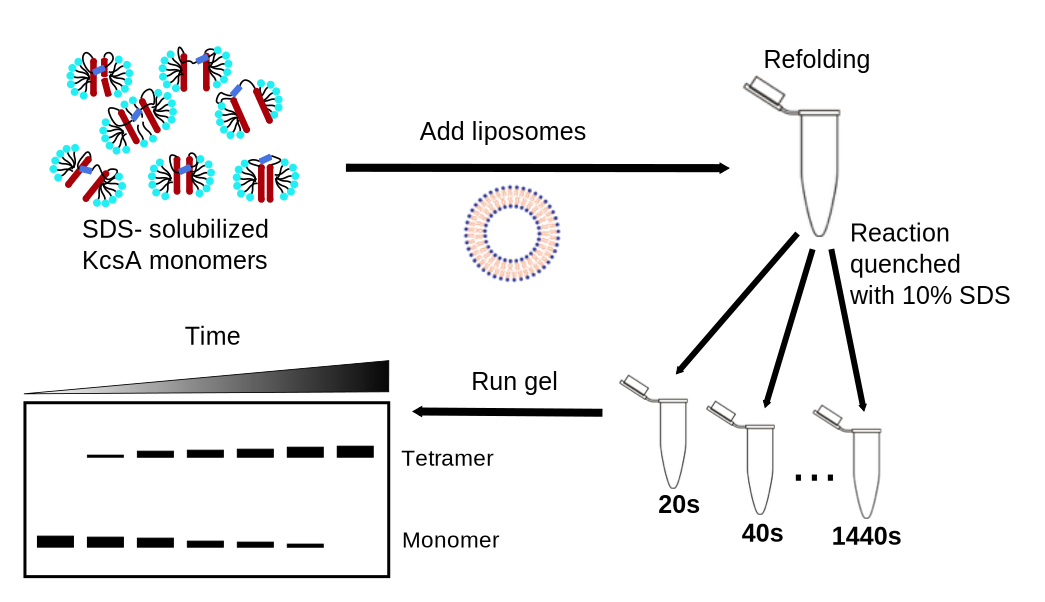
\includegraphics[width=\textwidth]{figures/chapter4/Fig4-1_refolding_protocol.pdf}
\end{center}
	\caption{\textbf{Structure of KcsA (PDB ID: 1R3J) shown from different angles}. \textbf{(A)} KcsA shown from the extracellular side of the membrane. \textbf{(B)} KcsA shown from the side. \textbf{(C)} KcsA viewed from the side with 2 monomers removed for better visualization of the selectivity filter. The oxygen atoms lining the selectivity region is rendered in Licoriche mode and the protein structures are rendered in New Cartoon mode in VMD. Each monomer of KcsA is colored in grey, blue, orange and red.}
	\label{fig:ch4_f1}
\end{figure}

Prior to refolding, precipitated KcsA $\Delta$125 monomers were solubilized in 0.5\% SDS in Buffer B with roughly protein concentrations of ~1.8 mg/mL. To initiate refolding, the protein mixture was diluted 10-fold into the refolding buffer containing asolectin vesicles. Then, at each time point a small aliquot of the refolding mixture was taken out and the reaction was quenched by diluting into 10\% SDS in Buffer B at 1:2 ratio. These quenched reaction mixtures were then run on a Novex Tris-glycine 4 – 20\% SDS-PAGE gel (ThermoFisher).

\subsection{Kinetics analysis}
	For analysis, gel images were taken with a Bio-rad ChemiDoc instrument. Then, the image was processed using ImageLab software to enhance the contrast between the protein bands and the background. For quantifying tetramer to monomer ratio, ImageJ software’s gel analysis tool was used. Each lane was normalized to itself by calculating the $\frac{[Tetramer]}{[Tetramer]+[Monomer]}$ ratio. For fitting, a double exponential function in the form of
	\begin{equation} a-be^{-\frac{t}{c}}-de^{-\frac{t}{e}} \end{equation}
was used and fitted using Scipy.optimize package in python.

\subsection{F\"{o}rster resonance energy transfer (FRET) of KcsA in liposomes}
For the site of dye conjugation, L86 in KcsA was chosen. The L86C mutation was obtained using the QuickChange protocol. Protein was expressed and purified as discussed above. Conjugation of either Cy3 or Cy5 maleimide (Kerafast) was done by overnight incubation at 4 $^{\circ}$C. Excess dye molecules were removed by size-exclusion chromatography using Superdex 200 Increase column (\textbf{Fig. \ref{fig:ch4_f2}} 

\begin{figure}[!ht]
\begin{center}
	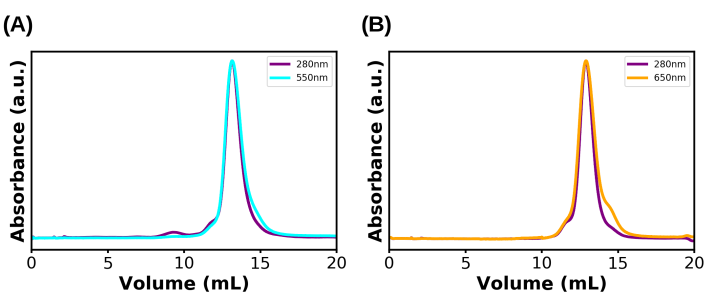
\includegraphics[width=\textwidth]{figures/chapter4/sec_cy3_cy5.pdf}
\end{center}
	\caption{\textbf{Structure of KcsA (PDB ID: 1R3J) shown from different angles}. \textbf{(A)} KcsA shown from the extracellular side of the membrane. \textbf{(B)} KcsA shown from the side. \textbf{(C)} KcsA viewed from the side with 2 monomers removed for better visualization of the selectivity filter. The oxygen atoms lining the selectivity region is rendered in Licoriche mode and the protein structures are rendered in New Cartoon mode in VMD. Each monomer of KcsA is colored in grey, blue, orange and red.}
	\label{fig:ch4_f2}
\end{figure}


Conjugation efficiency was calculated by the following equation:



\begin{equation}
	\mathrm{Conjugation\ Efficiency} = \frac{\epsilon_{dye}\alpha_{dye}}{\epsilon_{prot}\alpha_{280nm}+\epsilon_{dye}\alpha_{dye}}
\end{equation}

where $\epsilon_{prot}$ for KcsA is 33,460 cm$^{-1}$ M$^{-1}$, $\epsilon_{dye}$ = 150,000 cm$^{-1}$ M$^{-1}$ for Cy3 and 250,000 cm$^{-1}$ M$^{-1}$ Cy5, respectively, and absorbances ($\alpha_{280nm}$, $\alpha_{dye}$) were measured at 280 nm for KcsA, 550 nm for Cy3 and 650 nm for Cy5. The conjugation efficiency for both Cy3 and Cy5 samples were calculated to be ~50\%. FRET measurements were conducted with a Horiba Fluorolog-3 machine with Synapse OE-CCD Array Detector with an excitation wavelength $\lambda_{Ex}$= 500 nm. All samples contained 10 mg/mL SoyPC lipids with varying concentrations of proteins up to 10 $\mu$M.

\section{Results and Discussion}

\subsection{Kinetics of folding}

The kinetics of tetramerization of KcsA $\Delta$125 channels were examined by tracking the formation of native tetramers using an SDS resistance assay.31 The refolding protocol started with tricholoroacetic acid (TCA)-precipitated monomers solubilized with 14 mM (~0.5\% w/v) SDS at pH 6.5 (\textbf{Fig. \ref{fig:ch4_f1}A}). To initiate tetramerization, these monomers were diluted 10-fold into refolding buffer containing 14 mM asolectin liposomes. Control experiments employing dynamic light scattering verified that the liposomes remain intact after mixing with the SDS solubilized

KcsA $\Delta$125 or the 14 mM SDS buffer (Table. \ref{table:ch4_t1}). To measure refolding, aliquots of the protein-liposome mixture were removed over 25 minutes and quenched in 220 mM (~6\%) SDS buffer to arrest tetramer formation. At this high SDS concentration, liposomes were disrupted and only native tetramers persisted whereas weakly associated species were broken up and ran as monomers on SDS-PAGE gels.15-16, 31-32 The folding kinetics were quantified from the change in the gel band intensities.

\begin{table}[h]
\centering
	\caption{Folding monitored by SDS-Page gel.}
	\begin{tabular}{ccccc}
	\hline
           & WT $\Delta$125     & CC $\Delta$125      & WT FL     & CC FL                  \\
	\hline                                                                 
	\begin{tabular}[c]{@{}c@{}}Fast time\\ constant (s)\end{tabular} & \multicolumn{2}{c}{40 $\pm$ 2}     & \multicolumn{2}{c}{90 $\pm$ 10}     \\
Fast population    & \begin{tabular}[c]{@{}c@{}}0.25 $\pm$ 0.05 \\ (0.33 $\pm$ 0.05\\ 0.36 $\pm$ 0.05\\ 0.20 $\pm$ 0.05)\end{tabular} & \begin{tabular}[c]{@{}c@{}}0.86 $\pm$ 0.05\\ (0.86 $\pm$ 0.05\\ 0.83 $\pm$ 0.05\\ 0.87 $\pm$ 0.05)\end{tabular} & \begin{tabular}[c]{@{}c@{}}0.42 $\pm$ 0.04\\ (0.38 $\pm$ 0.04\\ 0.26 $\pm$ 0.04\\ 0 $\pm$ 0.04)\end{tabular} & \begin{tabular}[c]{@{}c@{}}0.55 $\pm$ 0.04\\ (0.44 $\pm$ 0.04\\ 0.16 $\pm$ 0.04\\ 0.13 $\pm$ 0.04)\end{tabular} \\
	\begin{tabular}[c]{@{}c@{}}Slow time\\ constant (s)\end{tabular} & \multicolumn{2}{c}{1500 $\pm$ 100} & \multicolumn{2}{c}{8400 $\pm$ 1600} \\
Slow population    & \begin{tabular}[c]{@{}c@{}}0.77 $\pm$ 0.03 \\ (0.70 $\pm$ 0.03\\ 0.68 $\pm$ 0.03\\ 0.83 $\pm$ 0.03)\end{tabular} & \begin{tabular}[c]{@{}c@{}}0.09 $\pm$ 0.03\\ (0.14 $\pm$ 0.03\\ 0.14 $\pm$ 0.03\\ 0.26 $\pm$ 0.03)\end{tabular} & \begin{tabular}[c]{@{}c@{}}0.59 $\pm$ 0.02\\ (0.63 $\pm$ 0.02\\ 0.76 $\pm$ 0.02\\ 1 $\pm$ 0.02)\end{tabular} & \begin{tabular}[c]{@{}c@{}}0.40 $\pm$ 0.02\\ (0.57 $\pm$ 0.02\\ 0.83 $\pm$ 0.02\\ 0.88 $\pm$ 0.02)\end{tabular} \\	\hline                
	\end{tabular}
	\label{table:ch4_t1}
	\end{table}
	
For KcsA $\Delta$125 monomers at 10 $\mu$M monomer concentration, two nearly equal refolding populations were observed, one that folded on sub-minute and another that folded on the 10 minute time scale (\textbf{Fig. \ref{fig:ch4_f3}}). Since the buildup of native tetramers is directly measured, the fast and slow appearance of native tetramers implies that there are multiple routes to the native state, rather than each phase representing a step on a sequential pathway, which would have resulted in a 10 minute lag in the buildup of tetramers.

\begin{figure}[!ht]
\begin{center}
	\includegraphics[width=\textwidth]{figures/chapter4/Fig4-2_kinetics.pdf}
\end{center}
	\caption{\textbf{Proposed KcsA folding and tetramerization.} SDS-solubilized monomers enter the liposomes and undergo rapid association into a protein-rich phase within the membrane prior to tetramerization. Oligomers can form with a native or non-native TM helical arrangement, which fold on the minute or 20 minute time scale, respectively, The rate limiting step on the faster pathway is proposed to involve the insertion of the pore helix to stabilize the tetramer in its native conformation.}
	\label{fig:ch4_f3}
\end{figure}

For the disulfide bonded CC construct, essentially all the monomers tetramerized at the fast rate (\textbf{Fig. \ref{fig:ch4_f3}}). This difference implied that the presence of unconstrained TM helices enabled the formation of a stably misfolded, slow folding species. Data for the WT and CC were fit globally, assuming the rates of the two phases were the same for the two versions. The resulting time constants were $\tau_{fast}$ = 40 $\pm$ 2 s and $\tau_{slow}$ = 1500 $\pm$ 100 s, with a 28 $\pm$ 6\% and 74 $\pm$ 6\% fast folding population for the WT and CC constructs, respectively.

\begin{figure}[!ht]
\begin{center}
	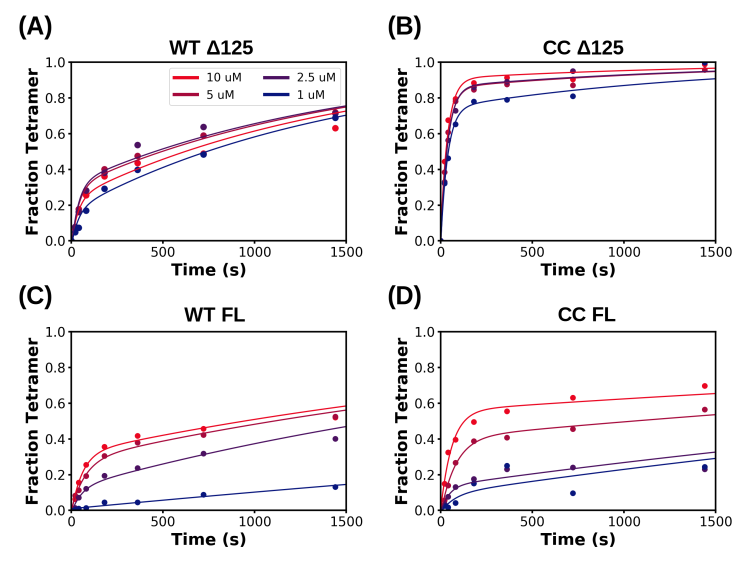
\includegraphics[width=\textwidth]{figures/chapter4/Fig4-3_conc_dependence.pdf}
\end{center}
	\caption{\textbf{Proposed KcsA folding and tetramerization.} SDS-solubilized monomers enter the liposomes and undergo rapid association into a protein-rich phase within the membrane prior to tetramerization. Oligomers can form with a native or non-native TM helical arrangement, which fold on the minute or 20 minute time scale, respectively, The rate limiting step on the faster pathway is proposed to involve the insertion of the pore helix to stabilize the tetramer in its native conformation.}
	\label{fig:ch4_f4}
\end{figure}

Next, the concentration dependence of the folding rates was studied. Interestingly, the tetramerization process, both in rate and branching ratio, appeared to be concentration independent from 1 to 10 $\mu$M within the accuracy of our measurements (\textbf{Fig. \ref{fig:ch4_f4}, Table. \ref{table:ch4_t1}}). This striking result indicates that the rate-limiting step in the folding process is a unimolecular process, despite the native state being a tetramer. If tetramerization was limited by the association of four monomers or two unstable dimers, one would have observed a 1000-fold slowing for a 10-fold decrease in concentration. As no measurable slowing was found, we propose that the oligomerization process occurs early and is fast on both routes, with the rate-limiting step representing a productive folding (fast pathway) or error-correction step (slow pathway). This proposal and the nature of this fast oligomerization process are investigated further with FRET below.

\subsection{FRET measurements suggest a formation of protein-rich phase}
The SDS folding assay indicated that the folding of both the WT and CC constructs has a minimal concentration dependence implying that the rate-limiting step is a unimolecular process. This step seems likely to occur after oligomerization in the liposomes. In principle, however, the insertion of monomers into the liposomes could be rate limiting. To test whether oligomerization is fast and occurs before the rate-limiting step, ensemble FRET measurements were carried out.

\begin{figure}[!ht]
\begin{center}
	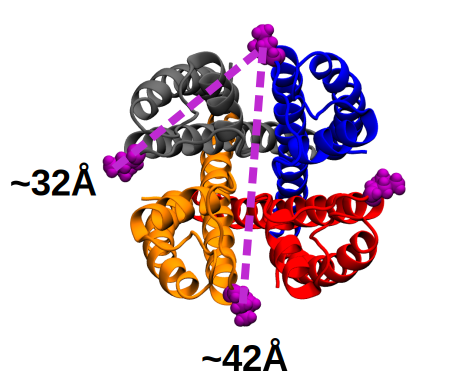
\includegraphics[width=8cm]{figures/chapter4/Fig4-4_fretpos.pdf}
\end{center}
	\caption{\textbf{Structure of KcsA with position L86C in purple.} Cy3 and Cy5 dyes were conjugated to position L86C, and mixed at a 1:1 ratio which results in two potential FRET distances of 32 and 42 Å.}
	\label{fig:ch4_f5}
\end{figure}

Dyes were first attached using thiol-labeling at a single position using a KcsA $\Delta$125 L86C variant (\textbf{Fig. \ref{fig:ch4_f5}}). Equal mixtures of donor (Cy3) and acceptor (Cy5) labeled KcsA $\Delta$125 were mixed and diluted 10-fold into the liposome mixture to initiate folding and the transfer of fluorescence was monitored (\textbf{Fig. \ref{fig:ch4_f6}}). Initially, the emission spectrum was dominated by that of the donor implying that most molecules began as isolated monomers. Upon dilution into a liposome mixture, the donor emission maximum at 570 nm was quenched by 71\% within the 10 second manual mixing dead-time while the acceptor’s emission at 680 nm increased by 7.6-fold. During the next 25 minutes over which tetramer formation occurred, only a 4\% increase in intensity was observed across the entire emission spectrum. 

\begin{figure}[!ht]
\begin{center}
	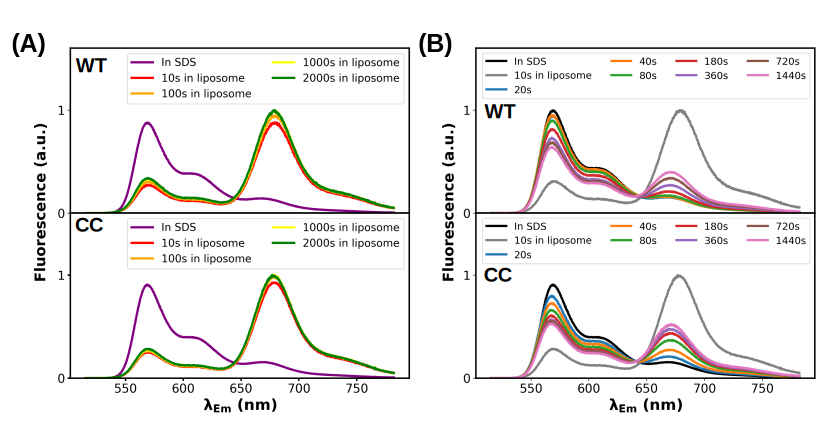
\includegraphics[width=\textwidth]{figures/chapter4/Fig4-5_fretdata.pdf}
\end{center}
	\caption{\textbf{FRET measurements of KcsA tetramerization.} \textbf{(A)} Ensemble FRET measurement of the KcsA monomer in SDS and in liposome as a function of time \textbf{(B)} Double-jump (unfold-fold-unfold) FRET measurements of KcsA refolding quenched with 10\% SDS overlaid with ‘in sds’ and ‘10s in liposome time points’ from \textbf{(A)}. Spectra are normalized to have the same value at 641 nm, an empirical iso-emissive point. Measurements are conducted at a monomer concentration of 10 $\mu$M.}
	\label{fig:ch4_f6}
\end{figure}

This biphasic FRET signal is interpreted as follows. The initial FRET increase indicates that the monomers labeled with donor and acceptor dyes rapidly associate in the liposomes prior to tetramerization. The minimal subsequent change implies that the FRET level in the rapidly associated monomers is similar to the level of folded tetramers in liposomes. The observation that most of the change in FRET signal occurred before significant tetramer formation, along with an estimate of $\sim$ 30 –- 300 monomers per liposome at 1 –- 10 $\mu$M monomer concentration, argues that most of the population forms a non-native oligomeric state upon insertion into liposomes with a FRET level comparable to that of native tetramers. The oligomers may become part of a protein-rich phase within the membrane.

To examine the possibility that FRET occurred within protein aggregates forming outside of liposomes, SDS-solubilized KcsA monomers were diluted 10-fold into water in the absence of liposomes. In this control, the overall donor fluorescence decreased 4\%, but the acceptor fluorescence spectrum only had a minimal indication of FRET (Fig. \ref), especially as compared to refolding in liposomes. The signal decrease indicates that some fraction of monomers was no longer in solution; however, more importantly, the lack of significant FRET indicates that the large observed FRET changes in the presence of liposome only came from membrane-solubilized proteins.

\begin{figure}[!ht]
\begin{center}
	\includegraphics[width=\textwidth]{figures/chapter4/Fig4-6_watercontrol.png}
\end{center}
	\caption{\textbf{FRET measurements of KcsA tetramerization.} \textbf{(A)} Ensemble FRET measurement of the KcsA monomer in SDS and in liposome as a function of time \textbf{(B)} Double-jump (unfold-fold-unfold) FRET measurements of KcsA refolding quenched with 10\% SDS overlaid with ‘in sds’ and ‘10s in liposome time points’ from \textbf{(A)}. Spectra are normalized to have the same value at 641 nm, an empirical iso-emissive point. Measurements are conducted at a monomer concentration of 10 $\mu$M.}
	\label{fig:ch4_f7}
\end{figure}

\section{Conclusion}

Our investigation of the folding of potassium channel monomers and their role in assembly of potassium channel pores revealed a number of salient features. The MD simulations and MSM analysis indicate that for both Kv1.2 pore domain and KcsA, monomers form a heterogeneous ensemble of native and non-native states with all three helices folded and lying within the membrane. While the population of native-like states of the monomer is non-negligible (18\% for Kv1.2 and 44\% for KcsA), it is nevertheless striking that a considerable number of non-native states exists despite the substantial conformational restriction imposed by the environment; namely, the secondary structure of all three helices is retained, and the two TM helices remain inserted within the planes of the bilayer. Based on prior studies of hydrophobic matching36-39, the different lengths of TM helices presumably contribute to their tendency to separate.

This overall picture is consistent with our NMR data combined with prior thiol-labeling studies.20-21 Our attempts to generate well-resolved NMR spectra for the WT KcsA monomer inserted in nanodisc and bicelles were unsuccessful. Suspecting that the separation of the TM helices was the critical feature, a double cysteine variant was engineered to have a disulfide bond at the bottom of the two TM helices locking them into a native-like arrangement. This CC variant yielded a well-dispersed 1H-15N HSQC spectrum supporting the view that the WT’s TM helices were often separated in the monomers and formed a heterogeneous ensemble.

FRET-monitored refolding measurements of monomers passing from SDS into liposomes indicated that both WT $\Delta$125 and CC $\Delta$125 variants oligomerized well before the appearance of native tetramers. According to both SDS-resistance assays and FRET measurements, WT KcsA monomers assembled into native tetramers via two distinct kinetic paths with 40  2 and 1500  100 s. The CC variant largely if not fully lacked the slow phase. We posit that slow folding is the result of non-native packing arrangements of the TM helices that must ultimately be corrected for tetrameric assembly to proceed. The observation of slow and fast folding routes has been seen in many soluble proteins where the initial collapse step leads to species with native-like topology on a direct pathway, or to a species containing a partially misfolded structure that is slow to correct (Fig. 5).40-42

\begin{figure}[!ht]
\begin{center}
	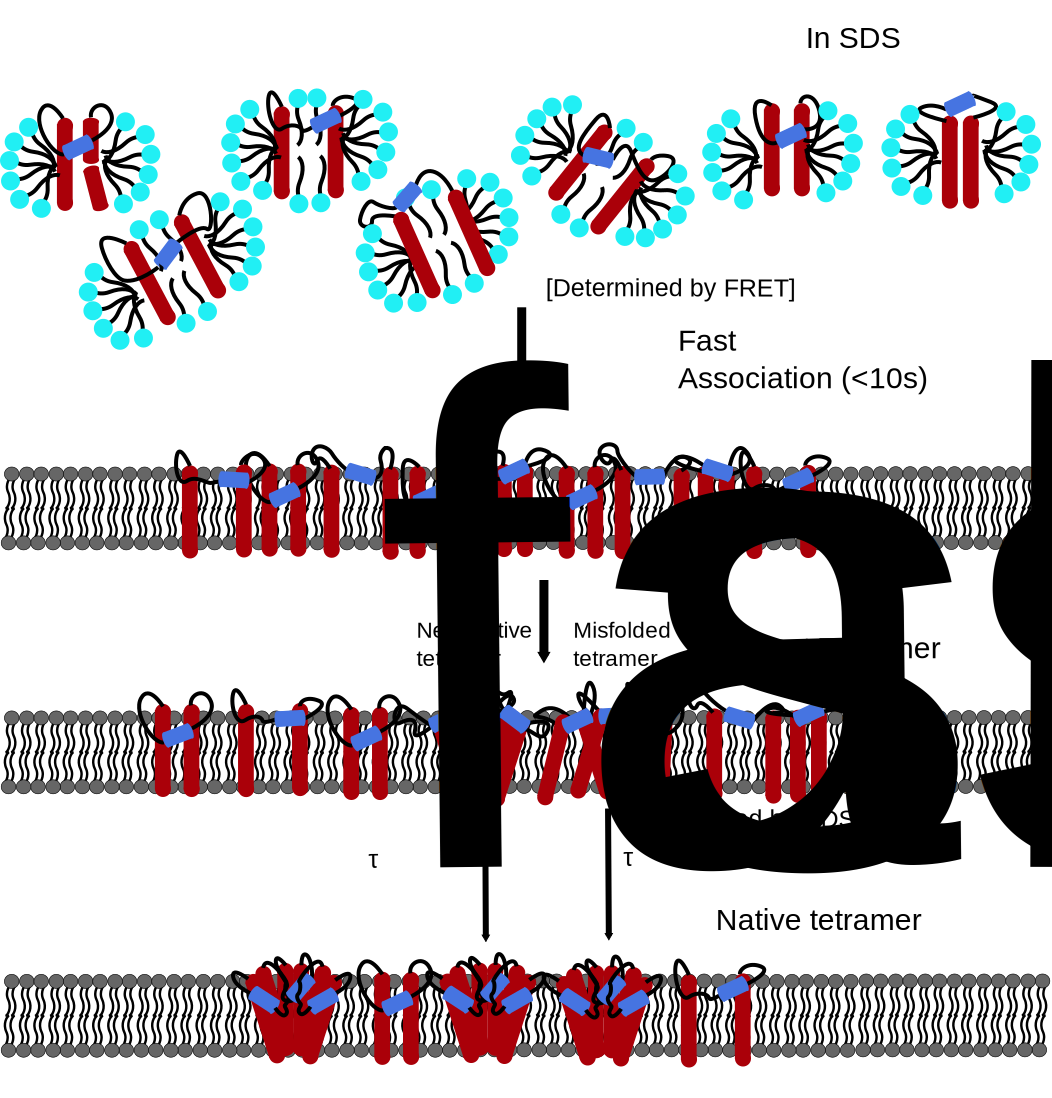
\includegraphics[width=\textwidth]{figures/chapter4/Fig4-7_summary.pdf}
\end{center}
	\caption{\textbf{Proposed KcsA folding and tetramerization.} SDS-solubilized monomers enter the liposomes and undergo rapid association into a protein-rich phase within the membrane prior to tetramerization. Oligomers can form with a native or non-native TM helical arrangement, which fold on the minute or 20 minute time scale, respectively, The rate limiting step on the faster pathway is proposed to involve the insertion of the pore helix to stabilize the tetramer in its native conformation.}
	\label{fig:ch4_f8}
\end{figure}

In spite of the channel being a tetramer, folding of the WT 125 and CC 125 constructs was concentration independent from 1 – 10 M for both the fast and slow phases, both in rate and amplitude. This observation implies that the rate-limiting step on both pathways is unimolecular. Because the FRET measurements indicated that the monomer insertion and oligomerization was relatively quick, the rate-limiting step on the fast pathway likely occurs going from an oligomer to a native tetramer. This complex transition requires the formation of the slightly twisted arrangement of the 8 TM helices, and the energetically costly opening of an aqueous channel. Final formation of native tetramers may occur in a concerted step with the association of correctly folded monomers already having the pore helices and selectivity filters positioned in a native or near-native orientation. Alternatively, this event may occur in two distinct steps, with the p-helices and selectivity filter segments folding into position only after the 8 TM have adopted their correct native arrangement. Further studies are needed to resolve this question.

The carboxy-terminal stalk domain in KcsA was tested to see if it enhanced tetramerization. In eukaryotic channels such as the Shaker voltage-activated potassium channel, the presence of the “tetramerization” T1 domain improves the rate of successful folding and assembly.13 Whereas the carboxy-terminal domain of KcsA forms a four-helix bundle that contributes to the stability of the folded tetrameric channel,43 its role in the assembly process is unclear. In other studies, the KcsA tetramerization domain alone has been shown to oligomerize in pH and concentration dependent manners44-45 as well as increase the stability of KcsA tetramers.33

However, the folding kinetics of KcsA pore domain with the tetramerization domain has not been extensively studied in the past. To our surprise, the presence of the tetramerization domain did not improve the channel’s folding behavior. For both the WT and CC variants, tetramerization became concentration dependent in a complex manner with both a reduced fast phase and lower overall yield of tetramers. One may consider that our refolding protocol with insertion into liposomes starting from an SDS-solubilized state does not properly mimic the biological context and so preclude the tetramerization domain for assisting folding. Also, the C-terminal region carries a net positive charge, which may cause a repulsion at large distance between monomers prior to tetramerization. Potentially the domain lends specificity and is more important for finding other KcsA subunits or improving the stability of tetramers once they are formed.

The folding of the potassium channels displays similar behavior to other -helical membrane proteins, having a transition state close to the native state.9-11 For example, in the force unfolding studies of GlpG pulling parallel to the bicelle surface, the transition state was closer to the native state than that observed in SDS-driven folding/unfolding studies in solution.46-47 In other SDS-based refolding studies on bacteriorhodopsin, DsbB and GlpG, the transition states were expanded.48-50 The observed difference between the force- and the SDS-driven unfolding studies may be due to the difference in the mode of denaturation as well as folding conditions (micelle or bicelle versus liposomes). Regardless, KcsA in liposomes appear to have a transition state near the native state.

The two-stage model, proposed nearly 30 years ago, has provided a useful framework for discussing membrane protein folding. The model, which posits insertion of all the TM helices followed by lateral packing, was proposed based on studies which observed that bacteriorhodopsin cut in a few pieces could still be re-assembled.51-53 With the observation of more diverse folding behaviors, a more sophisticated three-stage model10 was proposed where insertion and lateral packing of the TM helices could be followed by ligand binding, loop folding or peripheral domain insertion. This extra step is relevant to potassium channels, where the insertion of the four pore helices and the formation of the selectivity filter may be required to finalize the folding process.

For KcsA, the first two stages seem to correspond to insertion and formation of a protein-rich phase before folding into native tetrameric channels. This result brings up an interesting question in regards to membrane protein folding in general, namely, should the membrane be considered to be a good or poor solvent with respect to TM helices, defined as one where helix–lipid interactions are stronger or weaker, respectively, than helix–helix interactions. For potassium channels, a mixed behavior is observed. A protein-rich phase is detected by FRET, but the two TM helices in a monomer can dissociate from one other according to NMR (in bicelles) and MD simulations (POPC bilayers).

Potentially in the folding of other membrane proteins, non-specific or quinary interactions between TM helices also may give rise to a protein dense phase. These interactions can also occur in native structures, as seen with KcsA tetramers undergoing lateral association both in our and earlier studies.34-35 Several studies have shown that membrane proteins can alter lipid packing in the fluid liquid crystalline phase, which can in turn cause proteins to associate non-specifically in order to minimize the perturbation on the membrane.54-55 Generally, lipids may act as a marginally poor solvent for TM helices especially if the helices contain polar amino acids that are less soluble in the hydrophobic bilayer.56-62 These mixed results, along with variability of the hydrophobicity of the TM helices and the properties of the bilayer (e.g., composition, curvature, lateral pressure), suggest that solvent quality is likely system dependent. These issues have important implications to in vivo folding where helices partition between chamber of the translocon, lipid-water interface and the hydrophobic core of the membrane.63 

%% REVERT FIGURE NUMBERING %%
\renewcommand\thefigure{\thechapter.\arabic{figure}} 

%%% END CHAPTER 4 refolding studies %%%


%%% BEGIN CONCLUSION AND FUTURE DIRECTIONS %%%
\chapter{Conclusion and Future Directions}
\section{Conclusion}
This thesis provides the first comprehensive study on potassium channel folding. The dynamics of potassium channel monomers are first studied through MD simulations and NMR spectroscopy, through which we found that the potassium channel monomers are dynamical and exists in a heterogeneous ensemble of native and non-native structures. Although the exact population level is system dependent, we found that the native state is found in 18\% and 44\% for Kv1.2 and KcsA, respectively.

In order to design a mutant that remains its near-native state when monomerized, a disulfide-bridge was engineered at the ends of the 2 transmembrane helices in KcsA. By MD simulations and NMR spectroscopy, this disulfide-bonded (CC) KcsA mutant was shown to be more native-like and homogeneous in structural states.

In our folding kinetics studies of WT and CC KcsA, we found that WT folds via 2 distinct processes, whereas the CC variant only undergoes through the faster process. This result suggests that locking the 2 transmembrane helices in native-like arrangement reduces KcsA monomers to misfold, which allows this CC variant to fold only through the faster process. This type of biphasic folding kinetics has been seen in soluble proteins as well, where the faster kinetic process represents productive folding and the slower kinetic process represents error-prone or misfolding process.

In addition, concentration dependent folding kinetics of WT and CC KcsA was studied, in which we found that both WT and CC KcsA folding is concentration independent. This is quite surprising given that the native state of KcsA is a tetramer. For a simple kinetic scheme, $ 4 [M] \rightarrow [T]$, one would expect a 1000-fold decrease in $k_{app}$ or even if dimerization was rate-limiting, one would expect 10-fold decrease when monomer concentration is changed 10-fold. This result was surprising and suggested that the rate-limiting step in folding of ptoassium channel is unimolecular.

Our concentration dependent folding kinetics study led us to hypothesize that the oligomerization process could happen very early on and folding within this near-native state is what is rate-limiting in this folding reaction. In order to investigate whether if oligomerization indeed is quick, we utilized FRET. FRET results indicated that the oligomerization process is much quicker than folding reactions indicating that KcsA might form a non-specific interaction with each other to form a dense protein-rich phase.

\section{Future aims}
\subsection{Structure determination of disulfide engineered fast folding KcsA mutant}
The disulfide-bonded (CC) KcsA mutant was engineered to trap the KcsA monomers to be more native-like. Upon investigation of its kinetics, we found that this mutant folds more efficiently than the WT KcsA by avoiding misfolding of the 2 transmembrane helices. In addition, we found that the $^{1}$H-$^{15}$N-TROSY-HSQC spectrum looks much more folded than the WT spectrum. So, the question is what does the structure of this CC KcsA mutant look like in bicelles and what are its dynamics?

Through comparison of the folding kinetics of WT and CC KcsA variants we found that the misfolding of TM contributes to difference in folding kinetics between WT and CC KcsA. However, we still do not have a full understanding of how the arrangement of the pore helix affects the folding of KcsA. We hypothesize that the pore helix maintains its helicity and lay at the water-lipid interface. The pore helix maybe more dynamic than that potentially partitioning between multiple different states (solvent-exposed, lipid-water interface, and buried). With NMR peak assignments and structure, we can begin to answer some of the questions about the dynamics of the pore helix in membrane prior to tetramerization.

\subsection{Visualization of protein-rich phase}
The lipid raft hypothesis suggests that cholesterol and saturated lipids form preferential association in membranes and drive phase separation within the membrane. In return, this phase separation recruits other types of lipids and proteins for functional purposes and act as a way to compartmentalize within the membrane. In our FRET studies, we show that KcsA can non-specifically aggregate and form a protein-rich phase in the membrane.

In order to address the question of whether this protein-rich phase is real or not, we propose to use TIRF microscopy to study the formation of protein-rich phase. By looking at FRET under a microscope, we can directly observe whether protein-rich does occur in the membrane. In addition, this protein-rich phase seems to occur in soybean lipids, which we used in this thesis. It is possible that the soybean lipids act as poor solvent for KcsA causing the proteins to preferentially associate laterally in the membrane. Monitoring the formation of protein-rich phase under different lipid compositions will be informative. Perhaps, use of more anionic lipids or more unsaturated lipids can give rise to better solubilization of KcsA, which would eliminate the formation of protein-rich phase.

\subsection{Determination of the rate-limiting step in KcsA folding}
Through our concentration dependent folding kinetics studies, the rate-limiting step in KcsA folding was found to be unimolecular. This was quite surprising given the fact that KcsA is a tetramer in its native state. While we were able to show that by locking the 2 transmembrane helices in near-native state reduces KcsA's proclivity to misfold, the rate-limiting step in the reaction was not resolved.

We hypothesize that the rate-limiting step correponds to the insertion of pore helices into the chamber created by 8 transmembrane helices in the membrane. In order to test this hypothesis, here are some interesting ideas to try to pursue. 


%% END CONCLUSION AND FUTURE DIRECTIONS %%



% Format a LaTeX bibliography
\makebibliography

% Figures and tables, if you decide to leave them to the end
%\input{figure}
%\input{table}

\end{document}


